\section{Case Studies of Individual Sequences}
\label{sec:results/section_b}

In this section, we will look into tracking performance on the individual sequences to extend the analysis of all video sequences obtained in the previous section. Out of 12 video samples, we observed that most are consistent with the hypothesis that tracking performance scores decrease as QP increases, and the performance on the compressed sequences is lower than on uncompressed sequences. However, in some video samples, the performance scores increase midway through the QP range, but start decreasing at high QP, so it may happen that the performance on a compressed sequence with a moderate QP is better than the uncompressed one. These exceptional cases were observed in Cactus, BlowingBubbles, FourPeople, and KristenAndSara. To uncover the reason for this, we will examine the video samples: BasketballPass, Johnny, BlowingBubbles, and Cactus as case studies. Instead of tracking "all" object classes, we limit the tracking to the "person" object class in this analysis. The "person" object class is "cleaner" in terms of results than other classes, because the "person" class is more frequently present across the frames; in contrast, other object classes such as "sports ball" and "handbag" are rarely observed. We also included the "potted plant" class in Cactus. As different MSR did not impact the tracking performance according to the previous section, we selected MSR = 16 in the following analysis. Finally, we primarily focused on the MOTA score since this metric correlates the most with the human subjective impression of tracking according to \cite{leal-taixe_motchallenge_2015}. Since MOTA is defined in terms of FN, FP, and IDs from Equation \eqref{eqn:MOTA}, we will examine each of these metrics closely.


\subsection{BasketballPass}
We examined the results from the video sequence BasketballPass. This sequence consists of 7 "person" objects, and the occlusion frequently occurs in the video. Figure \ref{fig:BasketballPass_0_multiplots_qp} shows all the performance scores at different QPs at MSR = 16 and Table \ref{tab:BasketballPass_0} shows each numerical value. 
\begin{figure}[!htbp]
  \centering
  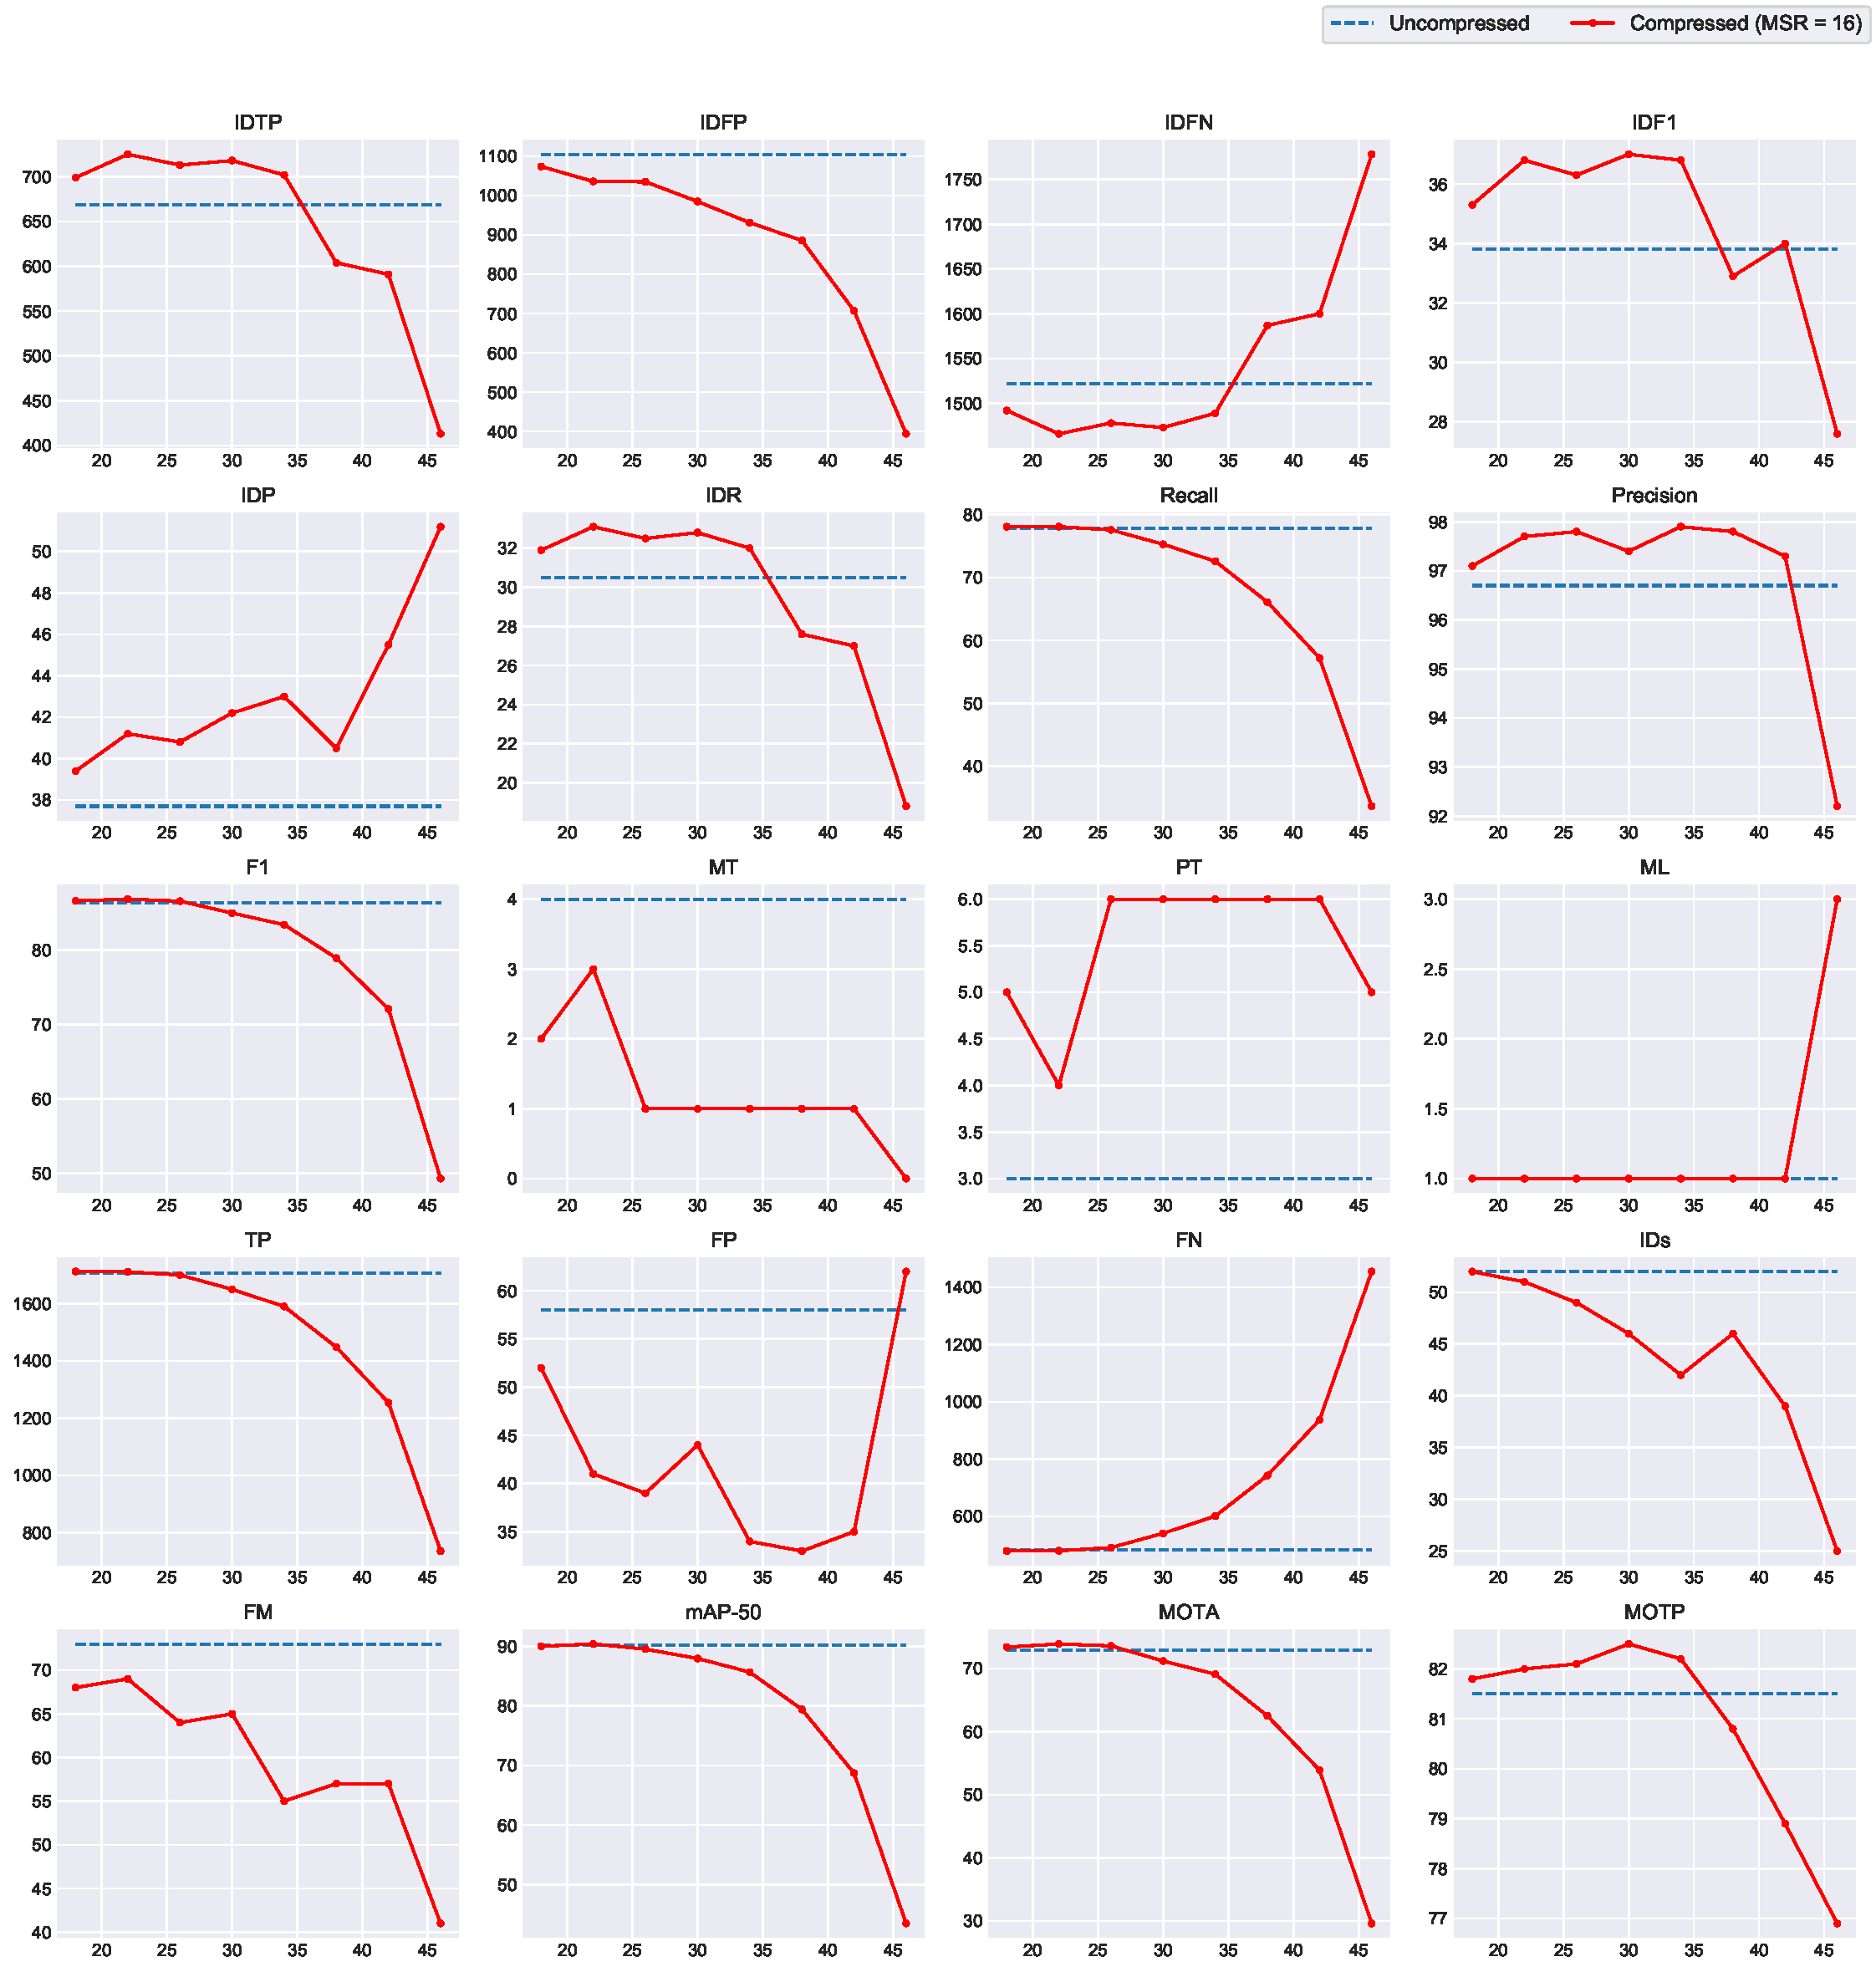
\includegraphics[width=1.0\linewidth]{img/BasketballPass_0_multiplots_qp.pdf}
  \caption[Visualization of the performance results in Class D BasketballPass at different QP for the "person" object class]
  {Visualization of the performance results in Class D BasketballPass at different QP for the "person" object class.
  }
  \label{fig:BasketballPass_0_multiplots_qp}
\end{figure}
\begin{table}[!tb]
    \centering
    \caption[Performance results on BasketballPass]
    {Performance results on BasketballPass.}
    \resizebox{1.0\linewidth}{!}{
\begin{tabular}{llrrrrrrrrrrrrrrrrrrrrr}
\toprule
          QP &          MSR &   IDTP &    IDFP &    IDFN &  IDF1 &   IDP &   IDR &  Recall &  Precision &    F1 &  GT &  MT &  PT &  ML &   TP &  FP &   FN &  IDs &  FM &  mAP-50 &  MOTA &  MOTP \\
\midrule
Uncompressed & Uncompressed & 669.00 & 1105.00 & 1522.00 & 33.80 & 37.70 & 30.50 &   77.90 &      96.70 & 86.29 &   8 &   4 &   3 &   1 & 1707 &  58 &  484 &   52 &  73 &   90.25 & 72.90 & 81.50 \\
          18 &           16 & 699.00 & 1074.00 & 1492.00 & 35.30 & 39.40 & 31.90 &   78.10 &      97.10 & 86.57 &   8 &   2 &   5 &   1 & 1712 &  52 &  479 &   52 &  68 &   90.03 & 73.40 & 81.80 \\
          22 &           16 & 725.00 & 1036.00 & 1466.00 & 36.80 & 41.20 & 33.10 &   78.10 &      97.70 & 86.81 &   8 &   3 &   4 &   1 & 1711 &  41 &  480 &   51 &  69 &   90.42 & 73.90 & 82.00 \\
          26 &           16 & 713.00 & 1035.00 & 1478.00 & 36.30 & 40.80 & 32.50 &   77.60 &      97.80 & 86.54 &   8 &   1 &   6 &   1 & 1700 &  39 &  491 &   49 &  64 &   89.54 & 73.60 & 82.10 \\
          30 &           16 & 718.00 &  985.00 & 1473.00 & 37.00 & 42.20 & 32.80 &   75.30 &      97.40 & 84.94 &   8 &   1 &   6 &   1 & 1650 &  44 &  541 &   46 &  65 &   87.98 & 71.20 & 82.50 \\
          34 &           16 & 702.00 &  931.00 & 1489.00 & 36.80 & 43.00 & 32.00 &   72.60 &      97.90 & 83.37 &   8 &   1 &   6 &   1 & 1590 &  34 &  601 &   42 &  55 &   85.69 & 69.10 & 82.20 \\
          38 &           16 & 604.00 &  886.00 & 1587.00 & 32.90 & 40.50 & 27.60 &   66.10 &      97.80 & 78.88 &   8 &   1 &   6 &   1 & 1448 &  33 &  743 &   46 &  57 &   79.42 & 62.50 & 80.80 \\
          42 &           16 & 591.00 &  707.00 & 1600.00 & 34.00 & 45.50 & 27.00 &   57.20 &      97.30 & 72.05 &   8 &   1 &   6 &   1 & 1254 &  35 &  937 &   39 &  57 &   68.72 & 53.90 & 78.90 \\
          46 &           16 & 413.00 &  394.00 & 1778.00 & 27.60 & 51.20 & 18.80 &   33.60 &      92.20 & 49.25 &   8 &   0 &   5 &   3 &  736 &  62 & 1455 &   25 &  41 &   43.45 & 29.60 & 76.90 \\
\bottomrule
\end{tabular}
    }
    \label{tab:BasketballPass_0}
\end{table}
The results are consistent with the average results shown in Section \ref{sec:results/section_a}, such that the performance decreases as QP increases on most of the metrics except IDP and MOTP. To examine the results more thoroughly, we inspected the video sequence frame by frame at different QP.
\begin{figure}[!tb]
  \centering
  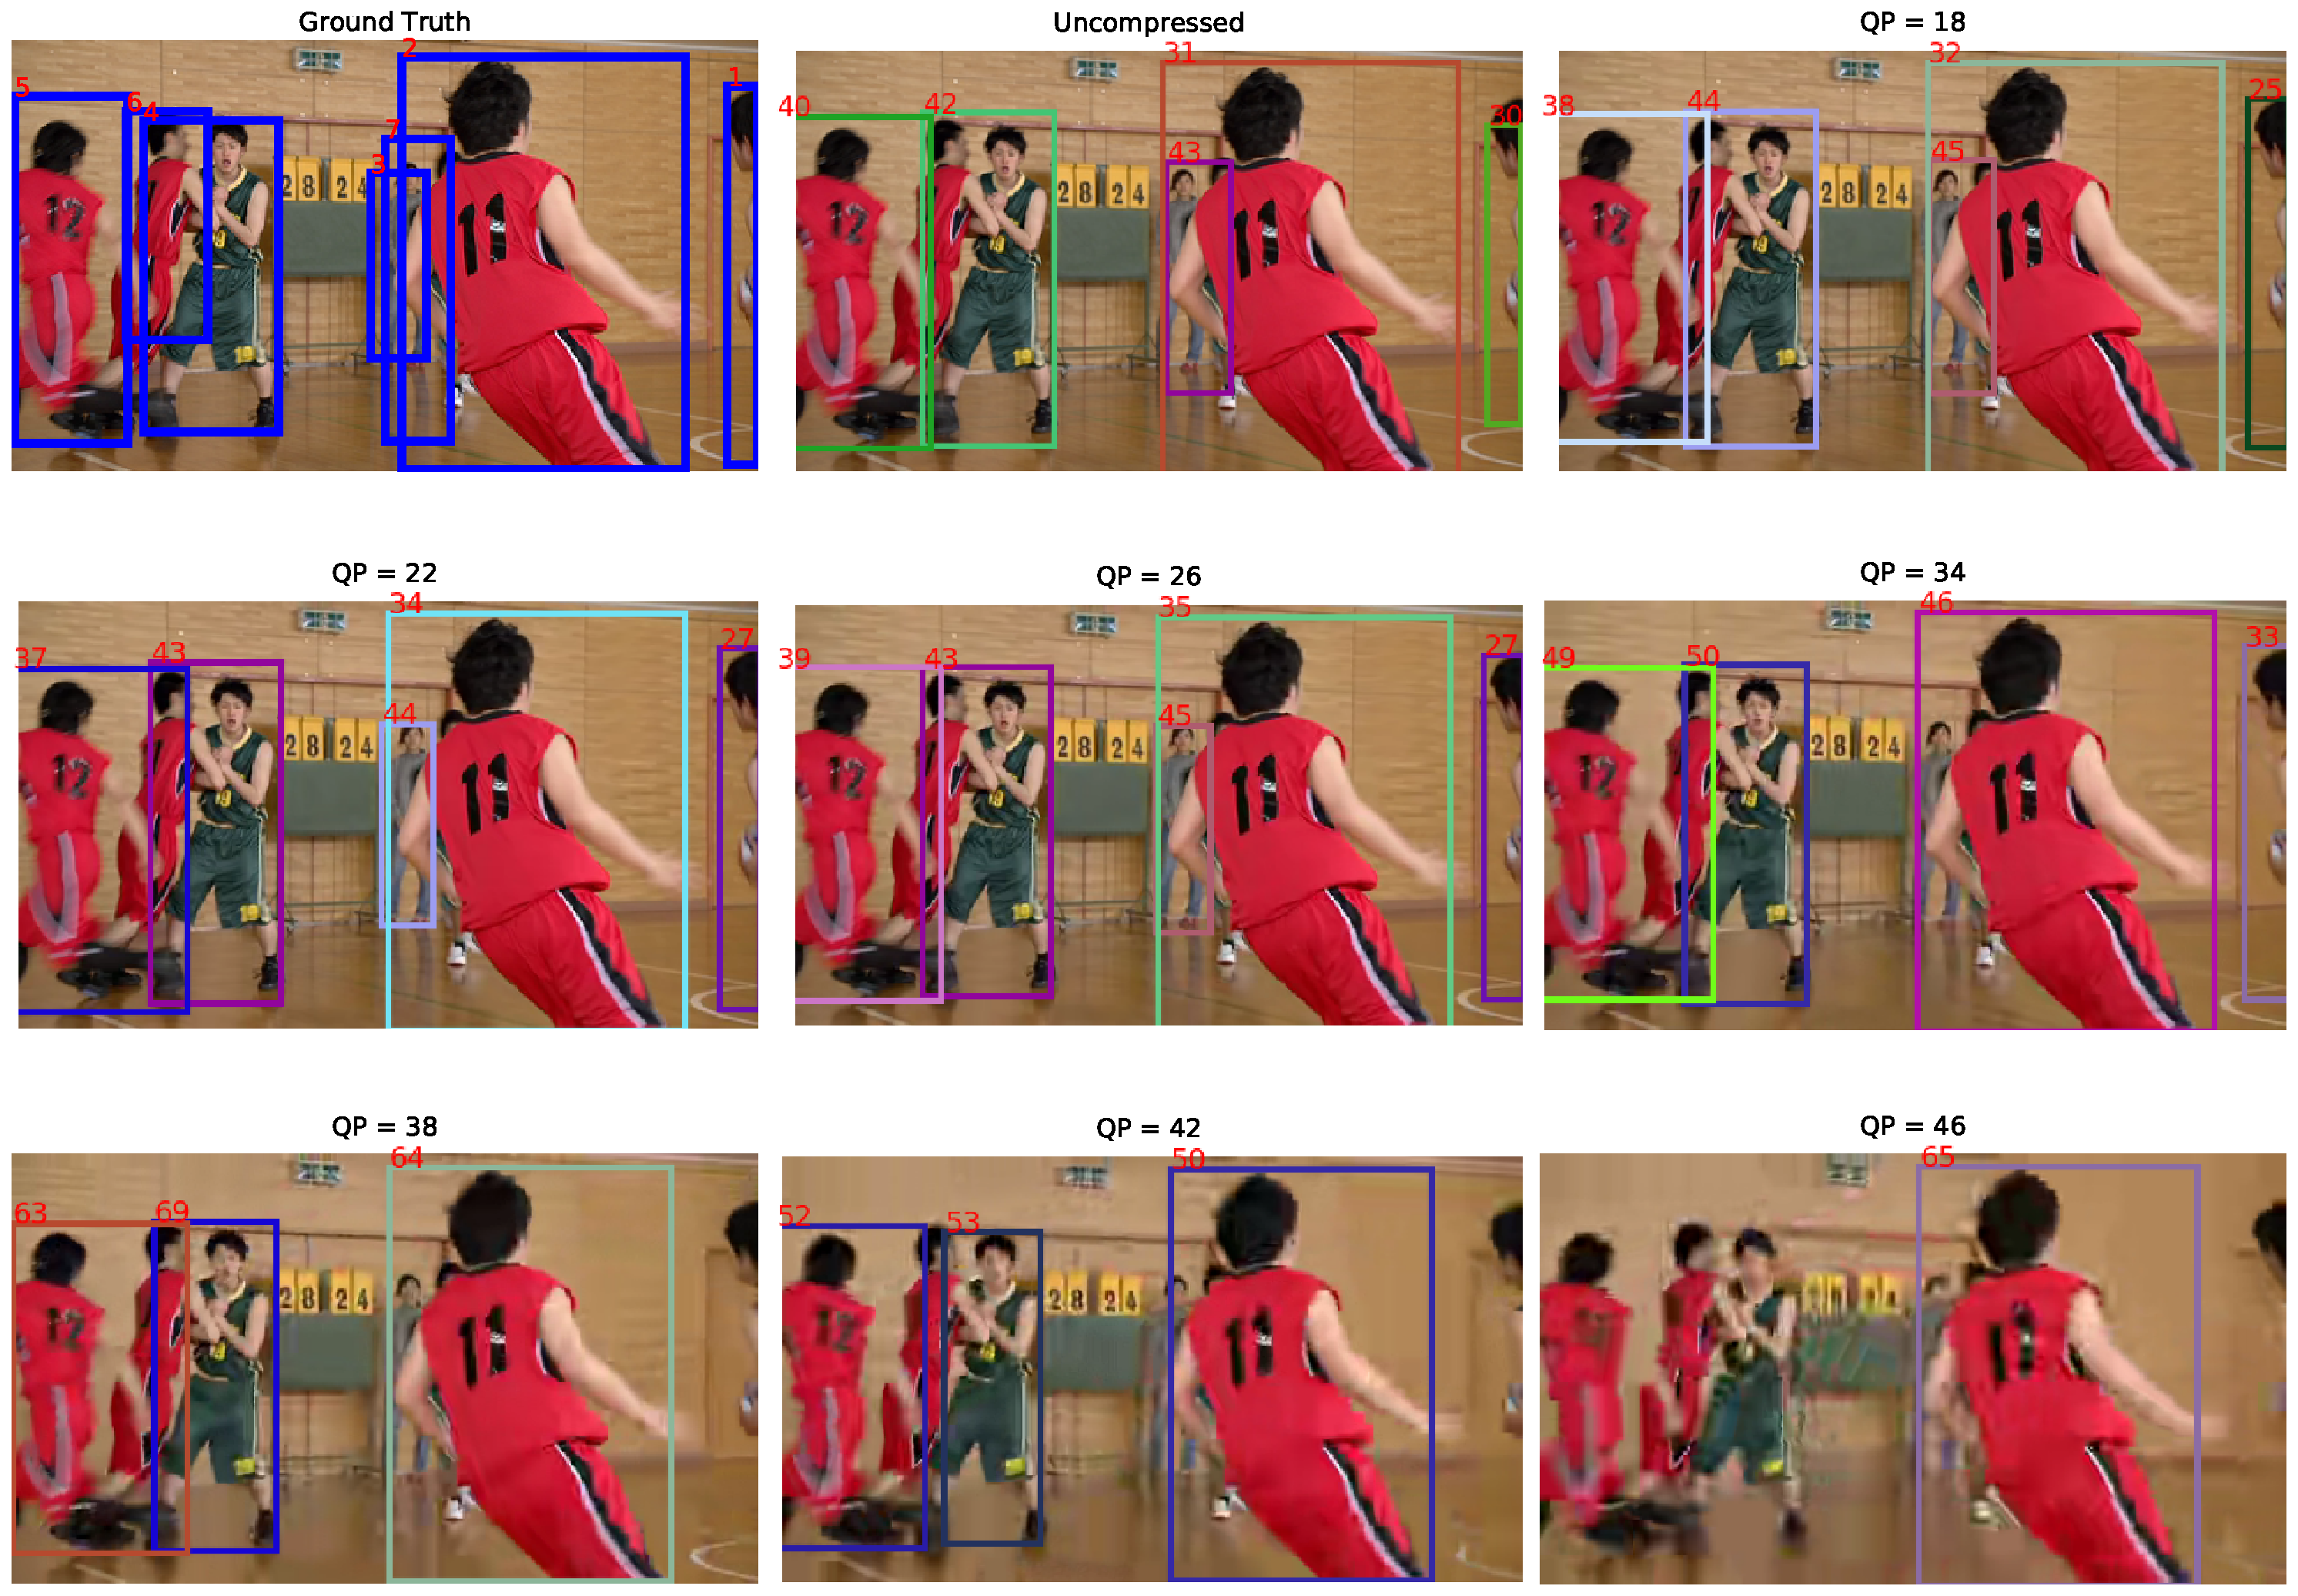
\includegraphics[width=1.0\linewidth]{img/BasketballPass_0_frame320.pdf}
  \caption[Comparison of ground truth and tracking results on the BasketballPass sequence in frames 320 at different QP]
  {
  Comparison of ground truth and tracking results on the BasketballPass sequence in frames at 320 at different QP.
  }
  \label{fig:BasketballPass_0_frame320}
\end{figure}
Figure \ref{fig:BasketballPass_0_frame320} shows the comparison of ground truth, tracking results without compression, and results with compression at different QP in the BasketballPass sequence at frame 320, as an example. This comparison illustrates that the higher the QP, the lower the image quality. As the quality decreases, the YOLOv3 detector starts failing to detect the "person" objects, and hence the FN increases. We also confirmed that IDs decreases because the number of detected objects decreases; therefore, the number of times the objects that are considered occluded also decreases. When the number of detected occlusion decreases, ID switch on the trajectories should decrease, since SORT does not have a feature to perform re-identification (re-ID) of the object identities. An example of this situation is shown in Figure \ref{fig:BasketballPass_0_IDs}.
\begin{figure}[!tb]
  \centering
  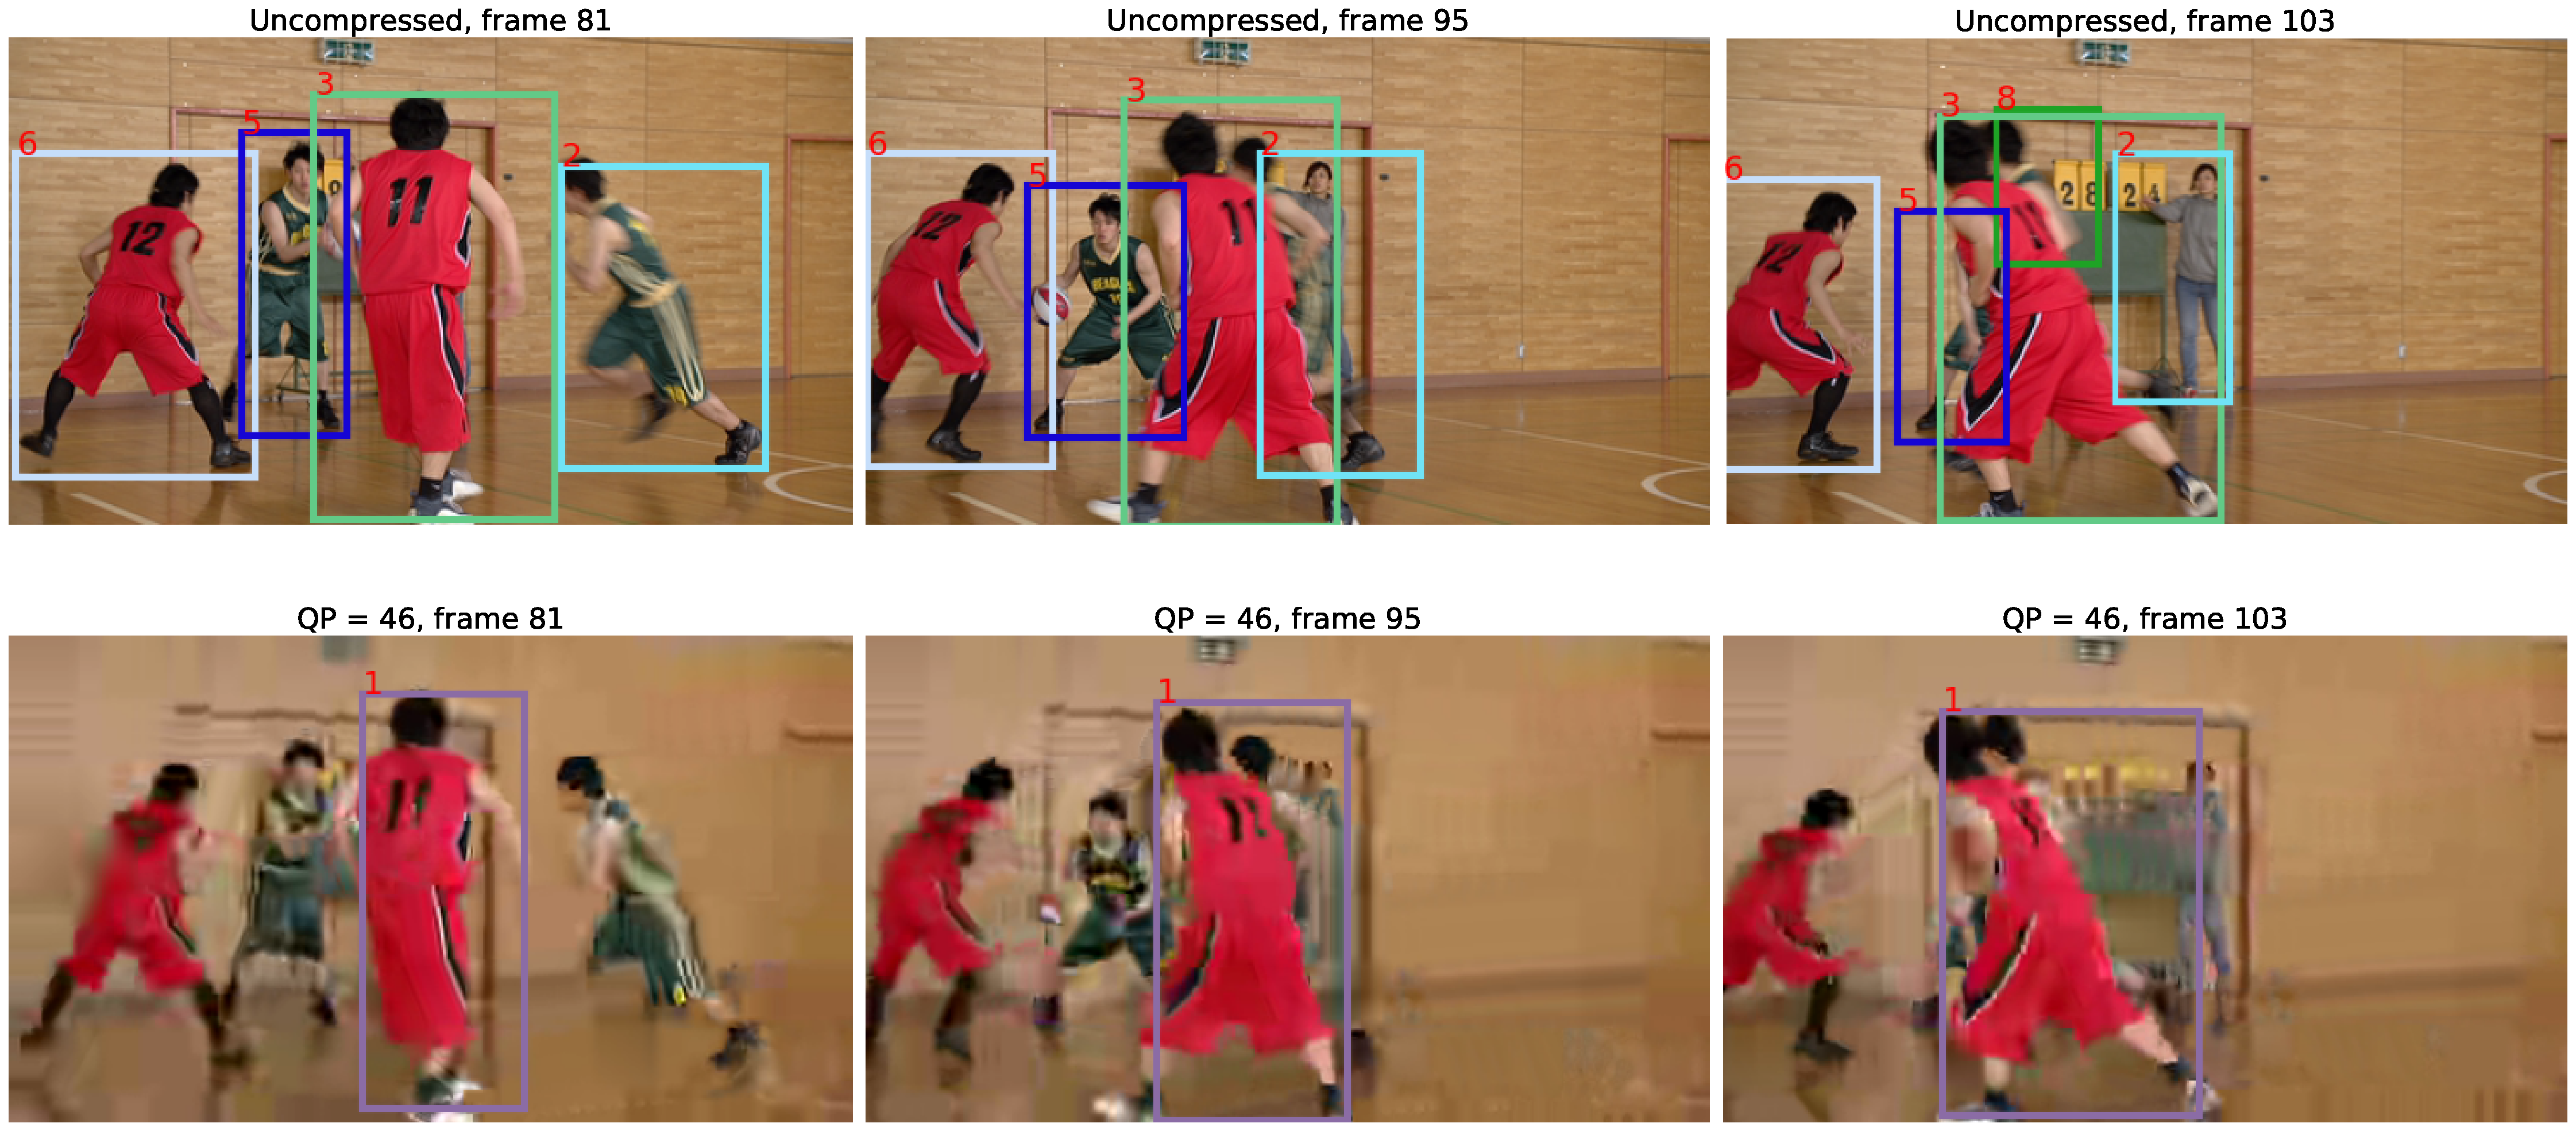
\includegraphics[width=1.0\linewidth]{img/BasketballPass_0_IDs.pdf}
  \caption[Comparison of BasketballPass frames 81, 95, 103 to explain IDs results]
  {
  Comparison of BasketballPass frames 81, 95, 103 to explain IDs results.
  }
  \label{fig:BasketballPass_0_IDs}
\end{figure}
The detected occlusion is shown in the uncompressed frames from 81 to 103, where the identities of two "person" objects are swapped due to occlusion. That same occlusion is not detected in the compressed frames at QP = 46. From FN, FP, and IDs, the increase of FN is significantly larger than the decrease of IDs and FP, so we conclude that MOTA decreases as QP increases based on Equation \eqref{eqn:MOTA}. 

From Figure \ref{fig:BasketballPass_0_multiplots_qp}, we observed that IDP increases. As we confirmed that the number of occlusions decreases as QP increases, we can verify that IDFP will also decrease. Hence, based on the IDP equation \eqref{eqn:IDP}, due to the drop of IDFP, IDP increases. This result can also be explained qualitatively as follows; as QP increases, the detected occlusion occurs less, so the incorrect ID assignments occur less, making ID precision higher at a higher QP.

\subsection{Johnny}
The Johnny sequence consists of 9 "person" objects. Occlusion was not observed, and the objects scarcely move. Figure \ref{fig:Johnny_0_multiplots_qp} shows a visualization of all the performance metrics at different QP, and Table \ref{tab:Johnny_0} shows the corresponding numerical values.
\begin{figure}[!tb]
  \centering
  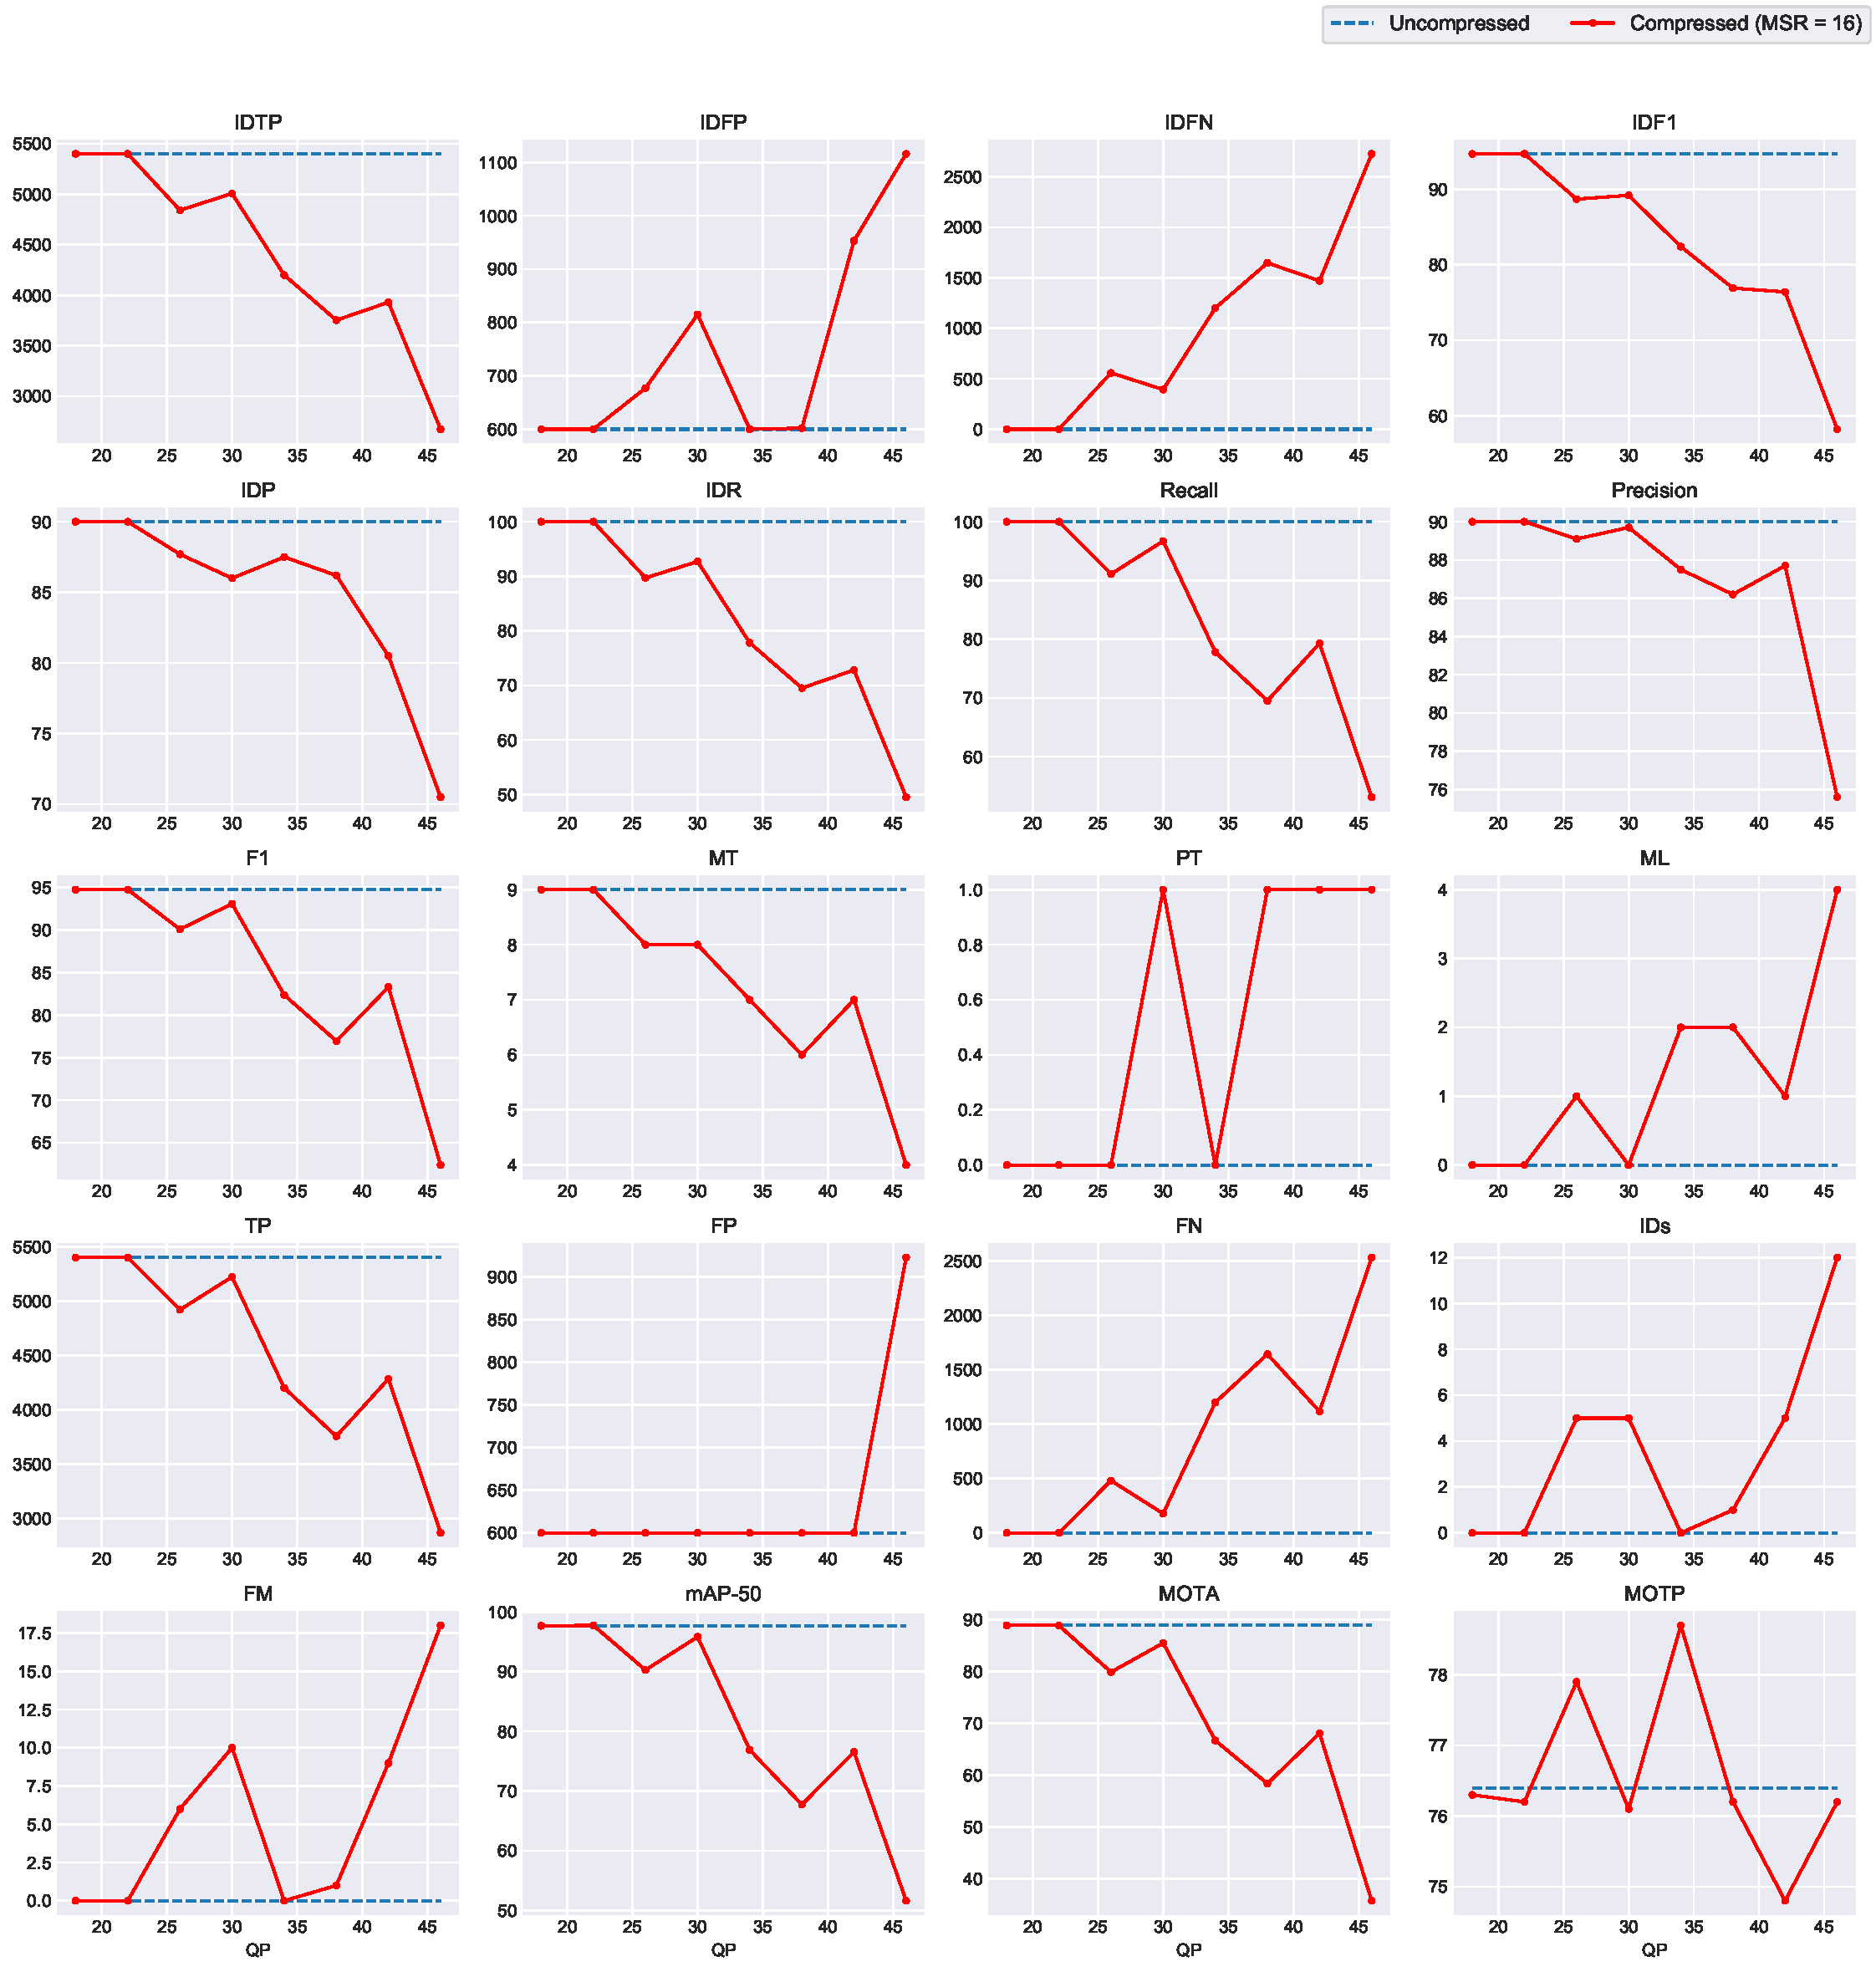
\includegraphics[width=1.0\linewidth]{img/Johnny_0_multiplots_qp.pdf}
  \caption[Visualization of the performance results on Johnny at different QP for the "person" object class]
  {
  Visualization of the performance results on Johnny at different QP for the "person" object class.
  }
  \label{fig:Johnny_0_multiplots_qp}
\end{figure}
\begin{table}[!tb]
    \centering
    \caption[Performance results on Johnny]
    {Performance results on Johnny.}
    \resizebox{1.0\linewidth}{!}{
\begin{tabular}{llrrrrrrrrrrrrrrrrrrrrr}
\toprule
          QP &          MSR &    IDTP &    IDFP &    IDFN &  IDF1 &   IDP &    IDR &  Recall &  Precision &    F1 &  GT &  MT &  PT &  ML &   TP &  FP &   FN &  IDs &  FM &  mAP-50 &  MOTA &  MOTP \\
\midrule
Uncompressed & Uncompressed & 5400.00 &  600.00 &    0.00 & 94.70 & 90.00 & 100.00 &  100.00 &      90.00 & 94.74 &   9 &   9 &   0 &   0 & 5400 & 600 &    0 &    0 &   0 &   97.72 & 88.90 & 76.40 \\
          18 &           16 & 5400.00 &  600.00 &    0.00 & 94.70 & 90.00 & 100.00 &  100.00 &      90.00 & 94.74 &   9 &   9 &   0 &   0 & 5400 & 600 &    0 &    0 &   0 &   97.70 & 88.90 & 76.30 \\
          22 &           16 & 5400.00 &  600.00 &    0.00 & 94.70 & 90.00 & 100.00 &  100.00 &      90.00 & 94.74 &   9 &   9 &   0 &   0 & 5400 & 600 &    0 &    0 &   0 &   97.76 & 88.90 & 76.20 \\
          26 &           16 & 4842.00 &  677.00 &  558.00 & 88.70 & 87.70 &  89.70 &   91.10 &      89.10 & 90.09 &   9 &   8 &   0 &   1 & 4919 & 600 &  481 &    5 &   6 &   90.29 & 79.90 & 77.90 \\
          30 &           16 & 5007.00 &  815.00 &  393.00 & 89.20 & 86.00 &  92.70 &   96.70 &      89.70 & 93.07 &   9 &   8 &   1 &   0 & 5222 & 600 &  178 &    5 &  10 &   95.85 & 85.50 & 76.10 \\
          34 &           16 & 4200.00 &  600.00 & 1200.00 & 82.40 & 87.50 &  77.80 &   77.80 &      87.50 & 82.37 &   9 &   7 &   0 &   2 & 4200 & 600 & 1200 &    0 &   0 &   76.89 & 66.70 & 78.70 \\
          38 &           16 & 3753.00 &  602.00 & 1647.00 & 76.90 & 86.20 &  69.50 &   69.50 &      86.20 & 76.95 &   9 &   6 &   1 &   2 & 3755 & 600 & 1645 &    1 &   1 &   67.73 & 58.40 & 76.20 \\
          42 &           16 & 3930.00 &  953.00 & 1470.00 & 76.40 & 80.50 &  72.80 &   79.30 &      87.70 & 83.29 &   9 &   7 &   1 &   1 & 4283 & 600 & 1117 &    5 &   9 &   76.54 & 68.10 & 74.80 \\
          46 &           16 & 2673.00 & 1116.00 & 2727.00 & 58.20 & 70.50 &  49.50 &   53.10 &      75.60 & 62.38 &   9 &   4 &   1 &   4 & 2866 & 923 & 2534 &   12 &  18 &   51.60 & 35.80 & 76.20 \\
\bottomrule
\end{tabular}
    }
    \label{tab:Johnny_0}
\end{table}
This result reveals that the most performance metrics decrease as QP increases similar to the case of BasketballPass. The decrease of performance can be verified from Figure \ref{fig:Johnny_0_frame400}, as the objects are starting to not be detected at higher QP values.
\begin{figure}[!htbp]
  \centering
  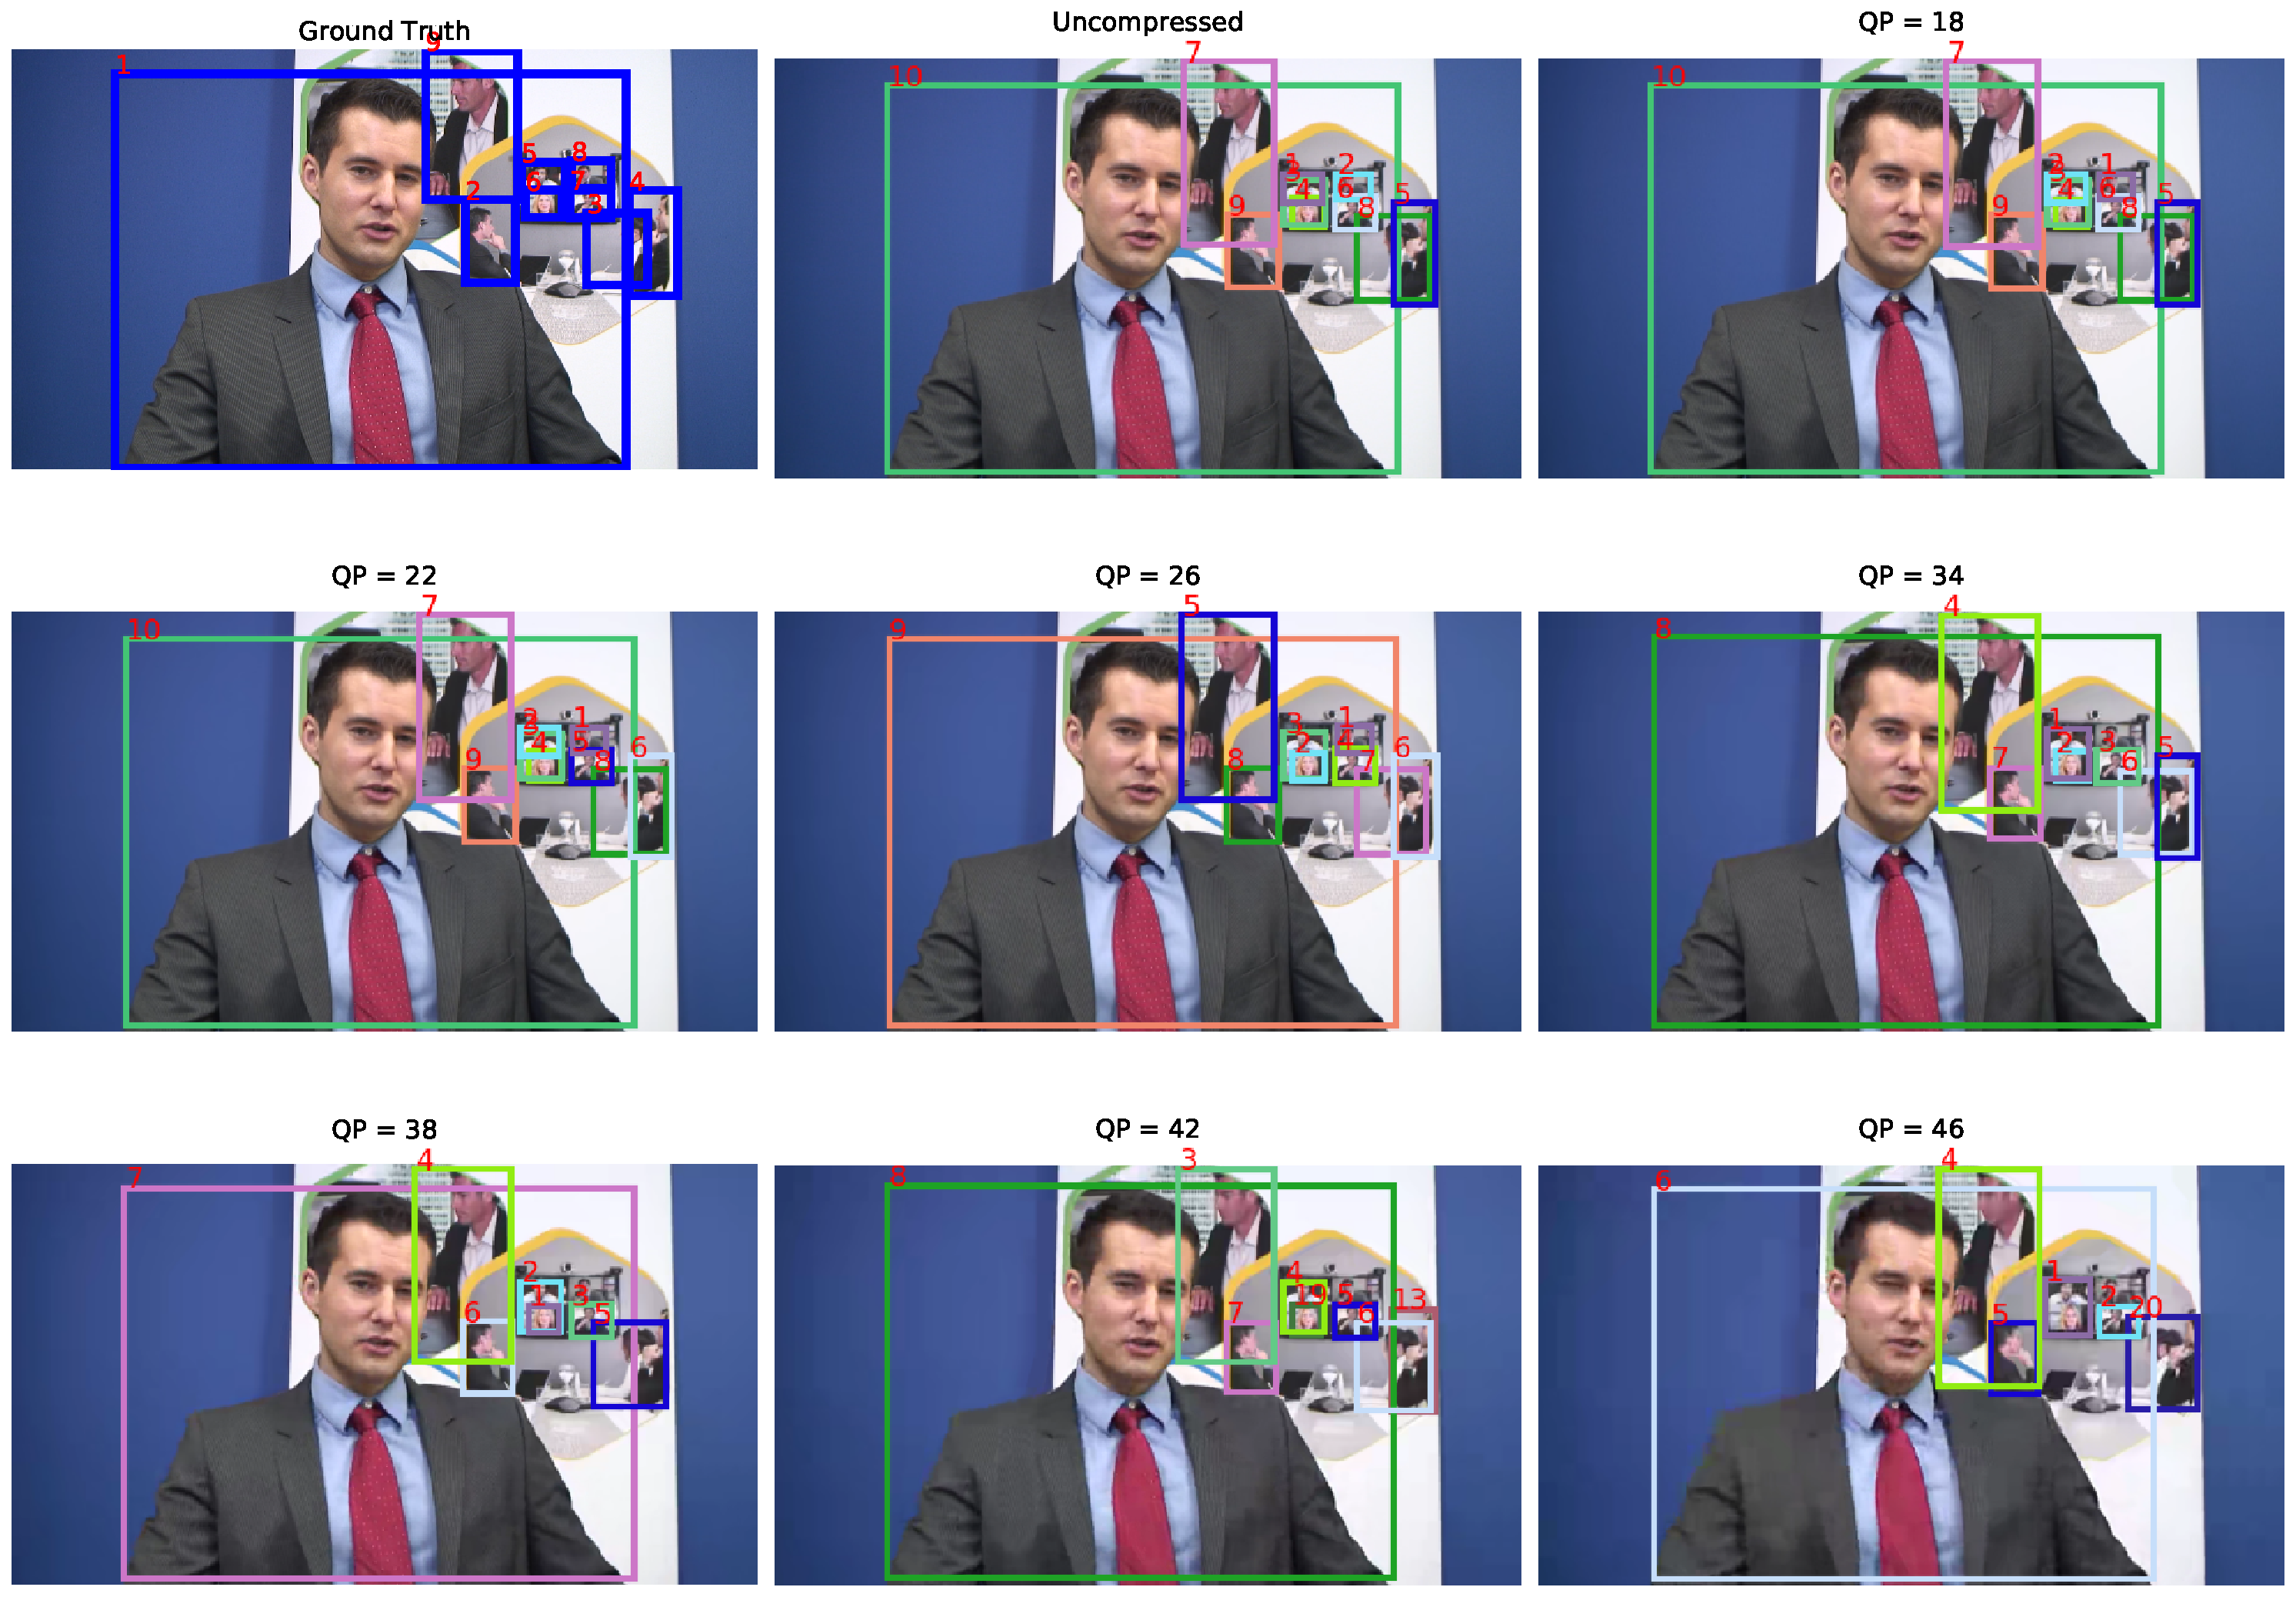
\includegraphics[width=1.0\linewidth]{img/Johnny_0_frame400.pdf}
  \caption[Comparison of Class E Johnny image frames at 320 at different QP]
  {
  Comparison of Class E Johnny image frames at 320 at different QP
  }
  \label{fig:Johnny_0_frame400}
\end{figure}
The decrease of detections explains the increase of FN. ID switch did not occur in the uncompressed sequence but was observed in the higher QP in the compressed sequence. Therefore, unlike in BasketballPass there is an increase in IDs at higher QP. The increase of IDs can be explained qualitatively as follows; since there is no occlusion in this sequence, ID switch between the trajectories does not occur at lower QP, but starts to occur at high QP as the image quality drops and different identities are assigned to the same trajectory. As the image quality drops, the objects starts to not be detected in some sequence of frames. As a result of "gap" in the trajectory, in other words, after a certain number of frames in which objects are not detected, different object identities are assigned to the targets after objects are detected again. Therefore, IDs increases as QP increases. As an example from Figure \ref{fig:Johnny_0_IDs}, the identity of one "person" object did not change in the uncompressed frames 282 to 290, but changed in the compressed frames at QP = 46.
\begin{figure}[!tb]
  \centering
  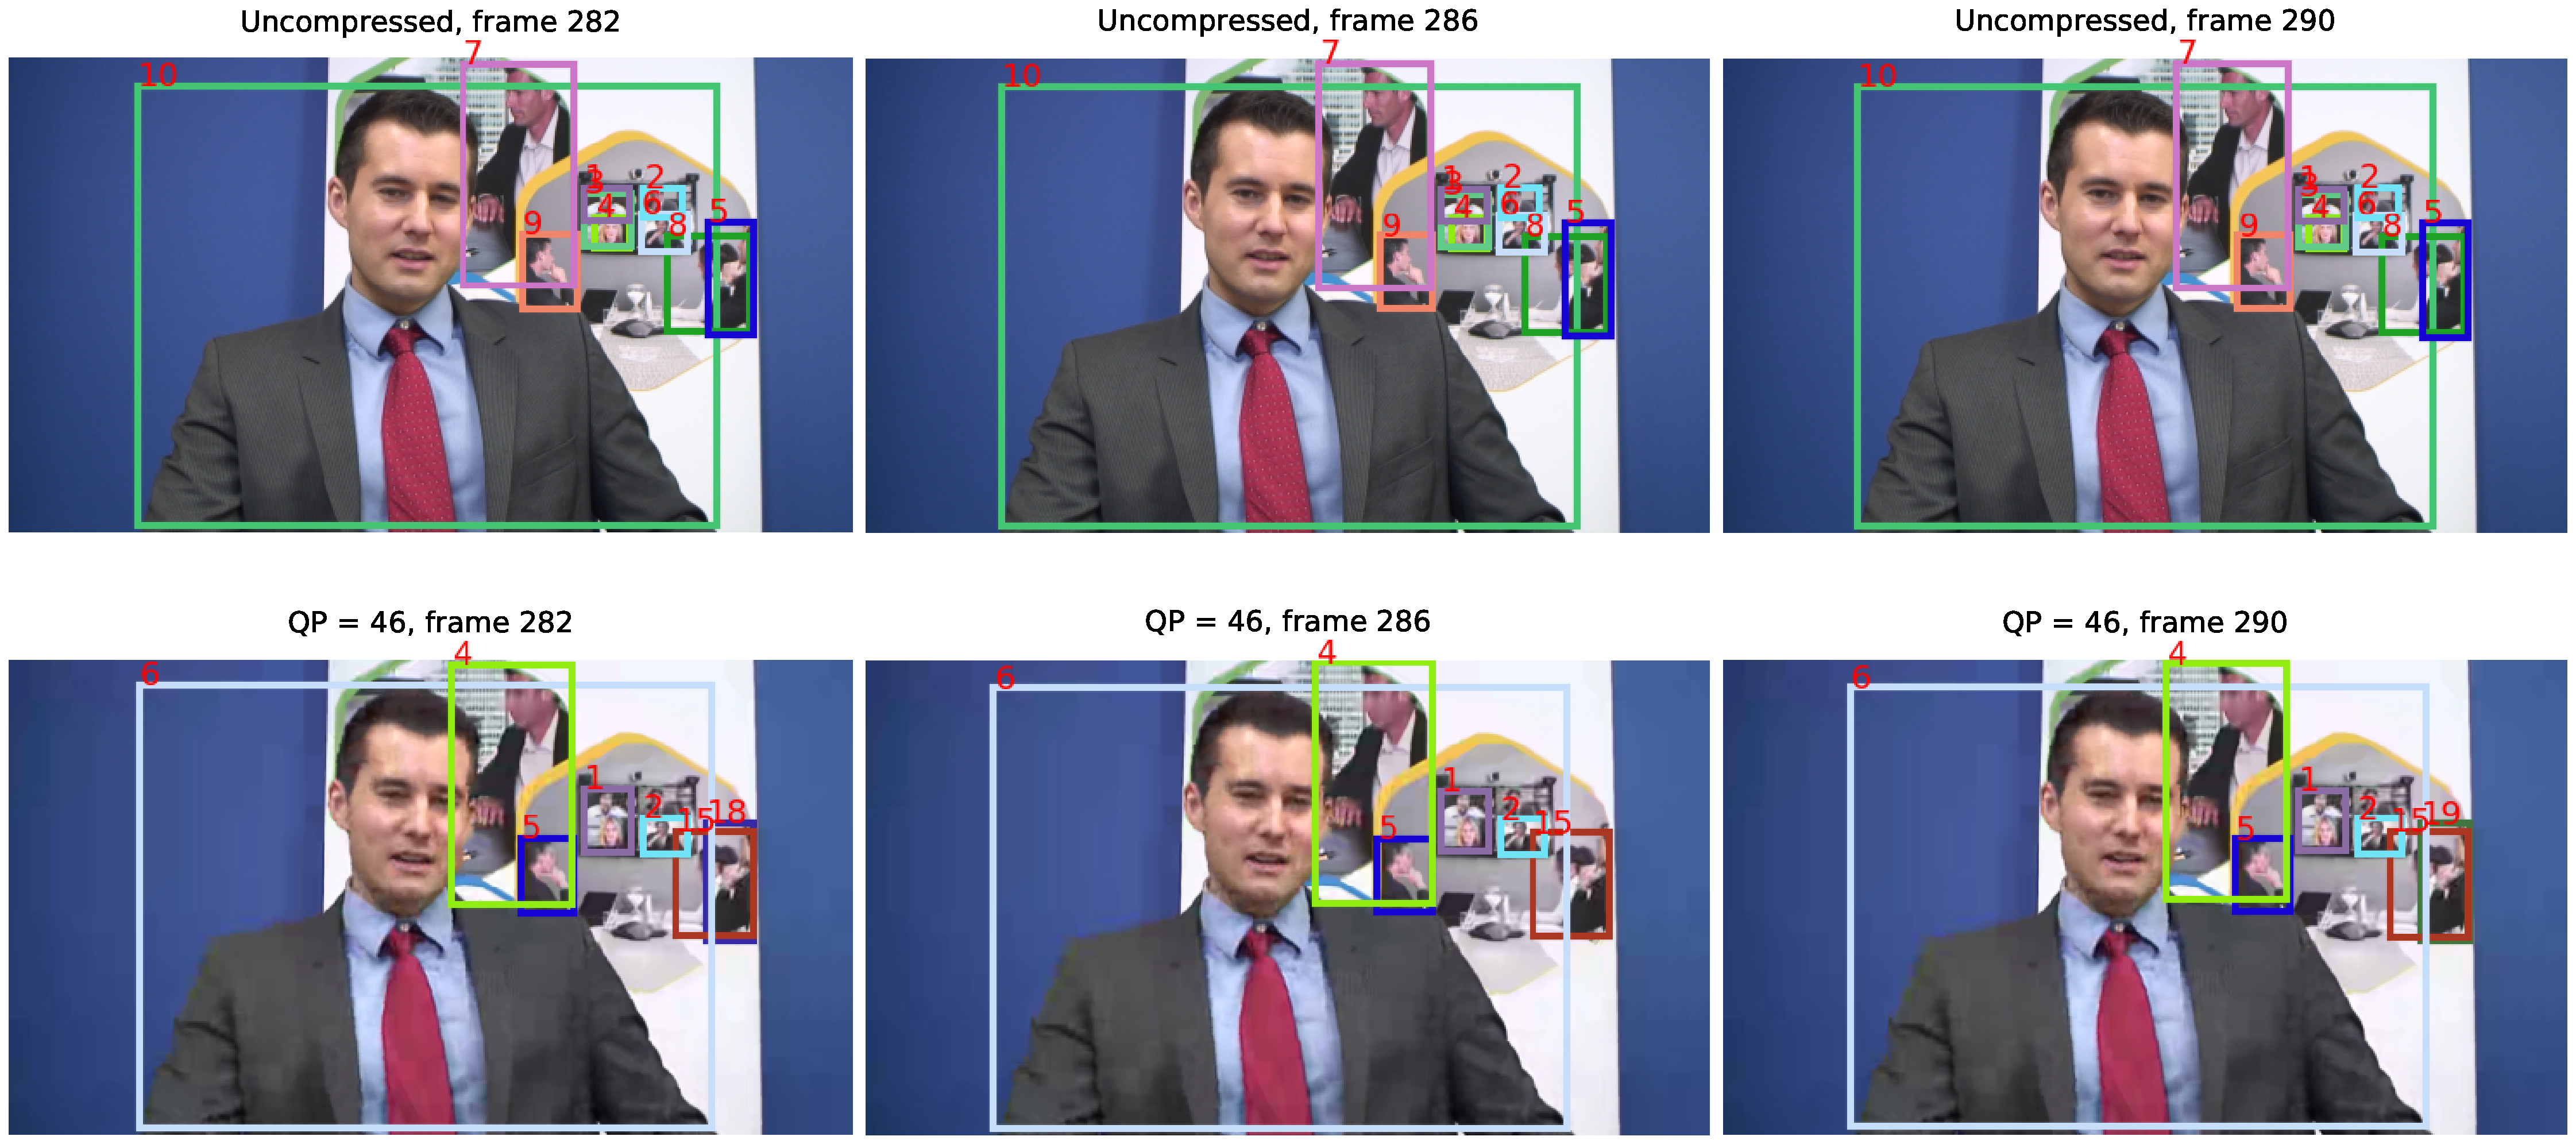
\includegraphics[width=1.0\linewidth]{img/Johnny_0_IDs.pdf}
  \caption[Comparison of Johnny frames 282, 286, 290 to explain IDs results]
  {
  Comparison of Johnny frames 282, 286, 290 to explain IDs results.
  }
  \label{fig:Johnny_0_IDs}
\end{figure}
Unlike the case of BasketballPass where the ID switch is caused by occlusion, ID switch in this sequence is caused by the "gap" in the trajectory, i.e., the detector fails to detect a particular object in a certain number of frames due to the drop of image quality in the trajectory but detect again. Based on all the increases of FP, FN, and IDs, the general tracking performance metric of MOTA decreases as QP increases.

Since IDs increases, we expect IDP to decrease. This is because the more ID switch occurs, the lower ID precision should be, and indeed IDR also decreases. The correlation between IDs and IDP is high, which can also be seen in Appendix \ref{sec:appendix/correlation}. Therefore, we confirmed that ID performance drops as QP increases. We also observed that other metrics such as detection performance and track quality drop as QP increases. The results in this sequence are different from the results on BasketballPass because the occlusion does not occur, so ID precision decreases as image quality drops.

\subsection{BlowingBubbles}
We will now examine the sequence where we observed an increase of MOTA with the increase of QP, which can be confirmed in the visualization in Figure \ref{fig:BlowingBubbles_0_multiplots_qp} and the numerical values in Table \ref{tab:BlowingBubbles_0}.
\begin{figure}[!tb]
  \centering
  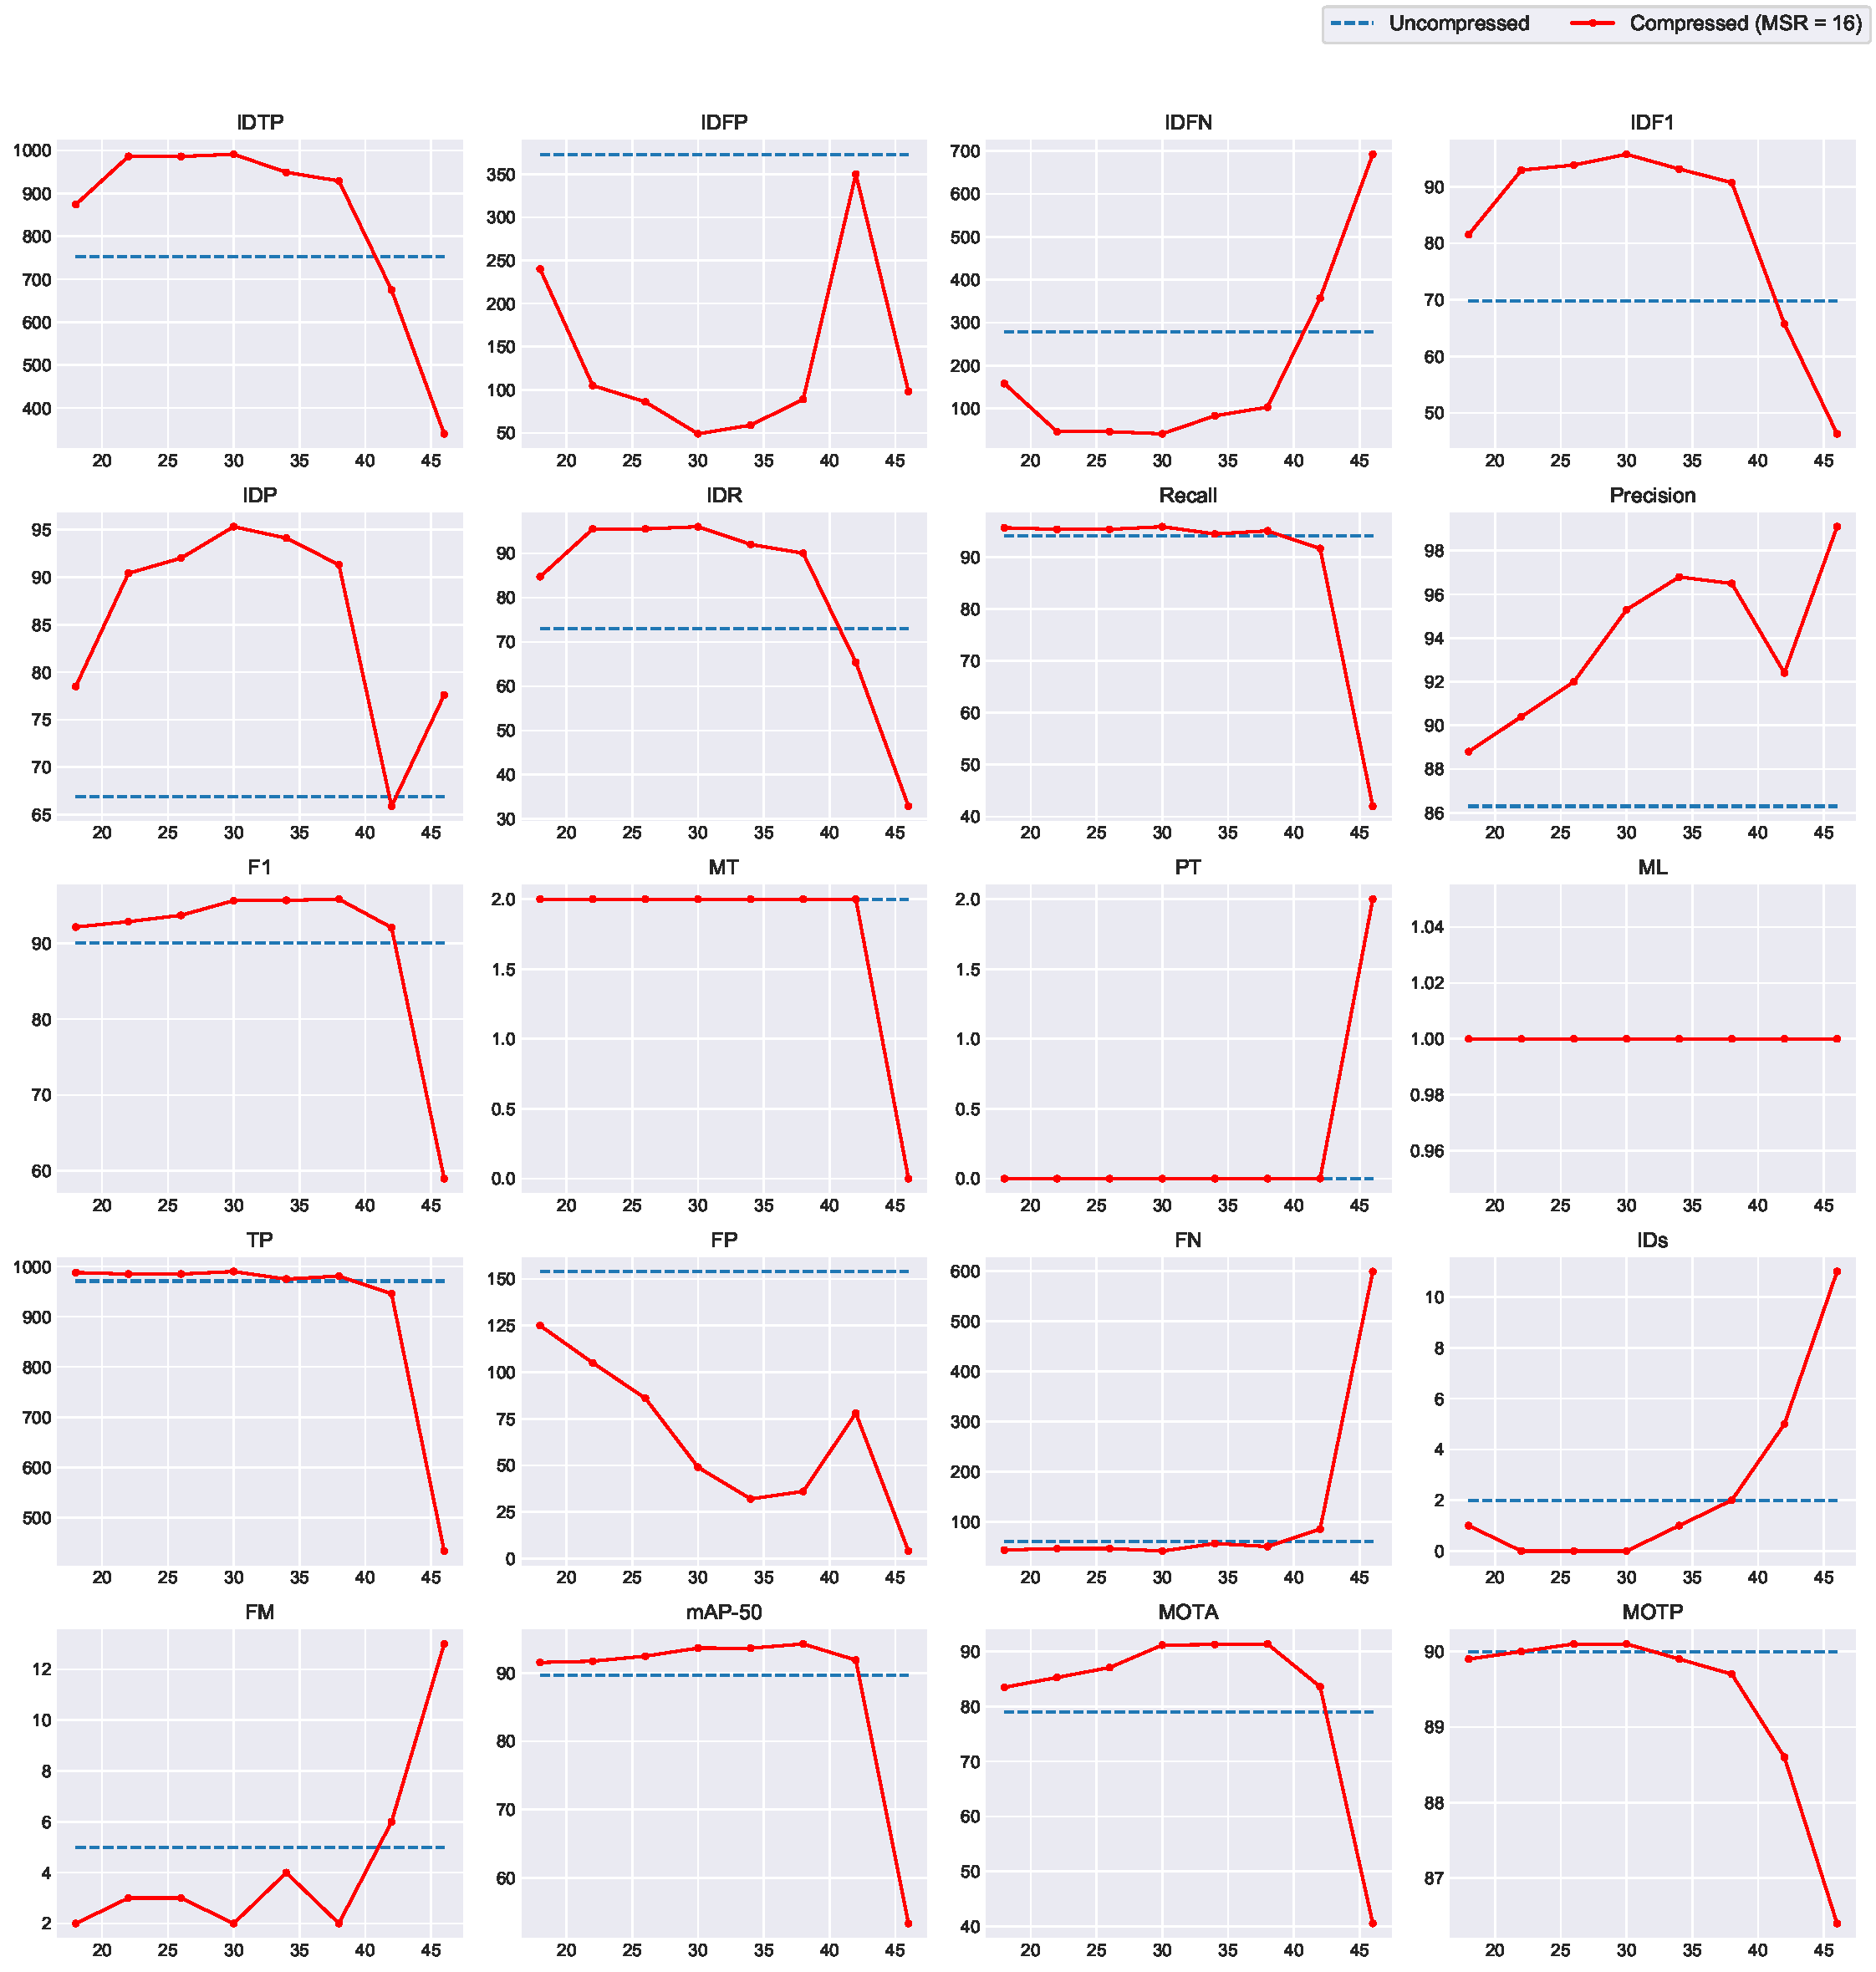
\includegraphics[width=1.0\linewidth]{img/BlowingBubbles_0_multiplots_qp.pdf}
  \caption[Visualization of the performance results on BlowingBubbles at different QP for the "person" object class]
  {
    Visualization of the performance results on BlowingBubbles at different QP for the "person" object class.
  }
  \label{fig:BlowingBubbles_0_multiplots_qp}
\end{figure}
\begin{table}[!htbp]
    \centering
    \caption[Performance results in Class D BlowingBubbles]
    {Performance results in Class D BlowingBubbles.}    \resizebox{1.0\linewidth}{!}{
    \begin{tabular}{llrrrrrrrrrrrrrrrrrrrr}
    \toprule
              QP &          MSR &   IDTP &   IDFP &   IDFN &  IDF1 &   IDP &   IDR &  Recall &  Precision &    F1 &  GT &  MT &  PT &  ML &  TP &  FP &  FN &  IDs &  FM &  MOTA &  MOTP \\
    \midrule
    Uncompressed & Uncompressed & 753.00 & 373.00 & 279.00 & 69.80 & 66.90 & 73.00 &   94.10 &      86.30 & 90.03 &   3 &   2 &   0 &   1 & 971 & 154 &  61 &    2 &   5 & 79.00 & 90.00 \\
              18 &           16 & 874.00 & 240.00 & 158.00 & 81.50 & 78.50 & 84.70 &   95.70 &      88.80 & 92.12 &   3 &   2 &   0 &   1 & 988 & 125 &  44 &    1 &   2 & 83.50 & 89.90 \\
              22 &           16 & 986.00 & 105.00 &  46.00 & 92.90 & 90.40 & 95.50 &   95.40 &      90.40 & 92.83 &   3 &   2 &   0 &   1 & 985 & 105 &  47 &    0 &   3 & 85.30 & 90.00 \\
              26 &           16 & 986.00 &  86.00 &  46.00 & 93.80 & 92.00 & 95.50 &   95.40 &      92.00 & 93.67 &   3 &   2 &   0 &   1 & 985 &  86 &  47 &    0 &   3 & 87.10 & 90.10 \\
              30 &           16 & 991.00 &  49.00 &  41.00 & 95.70 & 95.30 & 96.00 &   95.90 &      95.30 & 95.60 &   3 &   2 &   0 &   1 & 990 &  49 &  42 &    0 &   2 & 91.20 & 90.10 \\
              34 &           16 & 949.00 &  59.00 &  83.00 & 93.10 & 94.10 & 92.00 &   94.50 &      96.80 & 95.64 &   3 &   2 &   0 &   1 & 975 &  32 &  57 &    1 &   4 & 91.30 & 89.90 \\
              38 &           16 & 929.00 &  89.00 & 103.00 & 90.70 & 91.30 & 90.00 &   95.10 &      96.50 & 95.79 &   3 &   2 &   0 &   1 & 981 &  36 &  51 &    2 &   2 & 91.40 & 89.70 \\
              42 &           16 & 675.00 & 350.00 & 357.00 & 65.70 & 65.90 & 65.40 &   91.70 &      92.40 & 92.05 &   3 &   2 &   0 &   1 & 946 &  78 &  86 &    5 &   6 & 83.60 & 88.60 \\
              46 &           16 & 340.00 &  98.00 & 692.00 & 46.30 & 77.60 & 32.90 &   42.00 &      99.10 & 59.00 &   3 &   0 &   2 &   1 & 433 &   4 & 599 &   11 &  13 & 40.50 & 86.40 \\
    \bottomrule
    \end{tabular}
    }
    \label{tab:BlowingBubbles_0}
\end{table}
The MOTA visualization plot shows that the score increases until QP = 38 but decreases thereafter. To analyze this outcome, we inspected the video carefully frame by frame. From Figure \ref{fig:BlowingBubbles_0_frame465}, which shows frame 465, we observed a toy, a humanlike object, was detected as "person" in the uncompressed case and at QP = 18, 22, 26, but not thereafter.
\begin{figure}[!htbp]
  \centering
  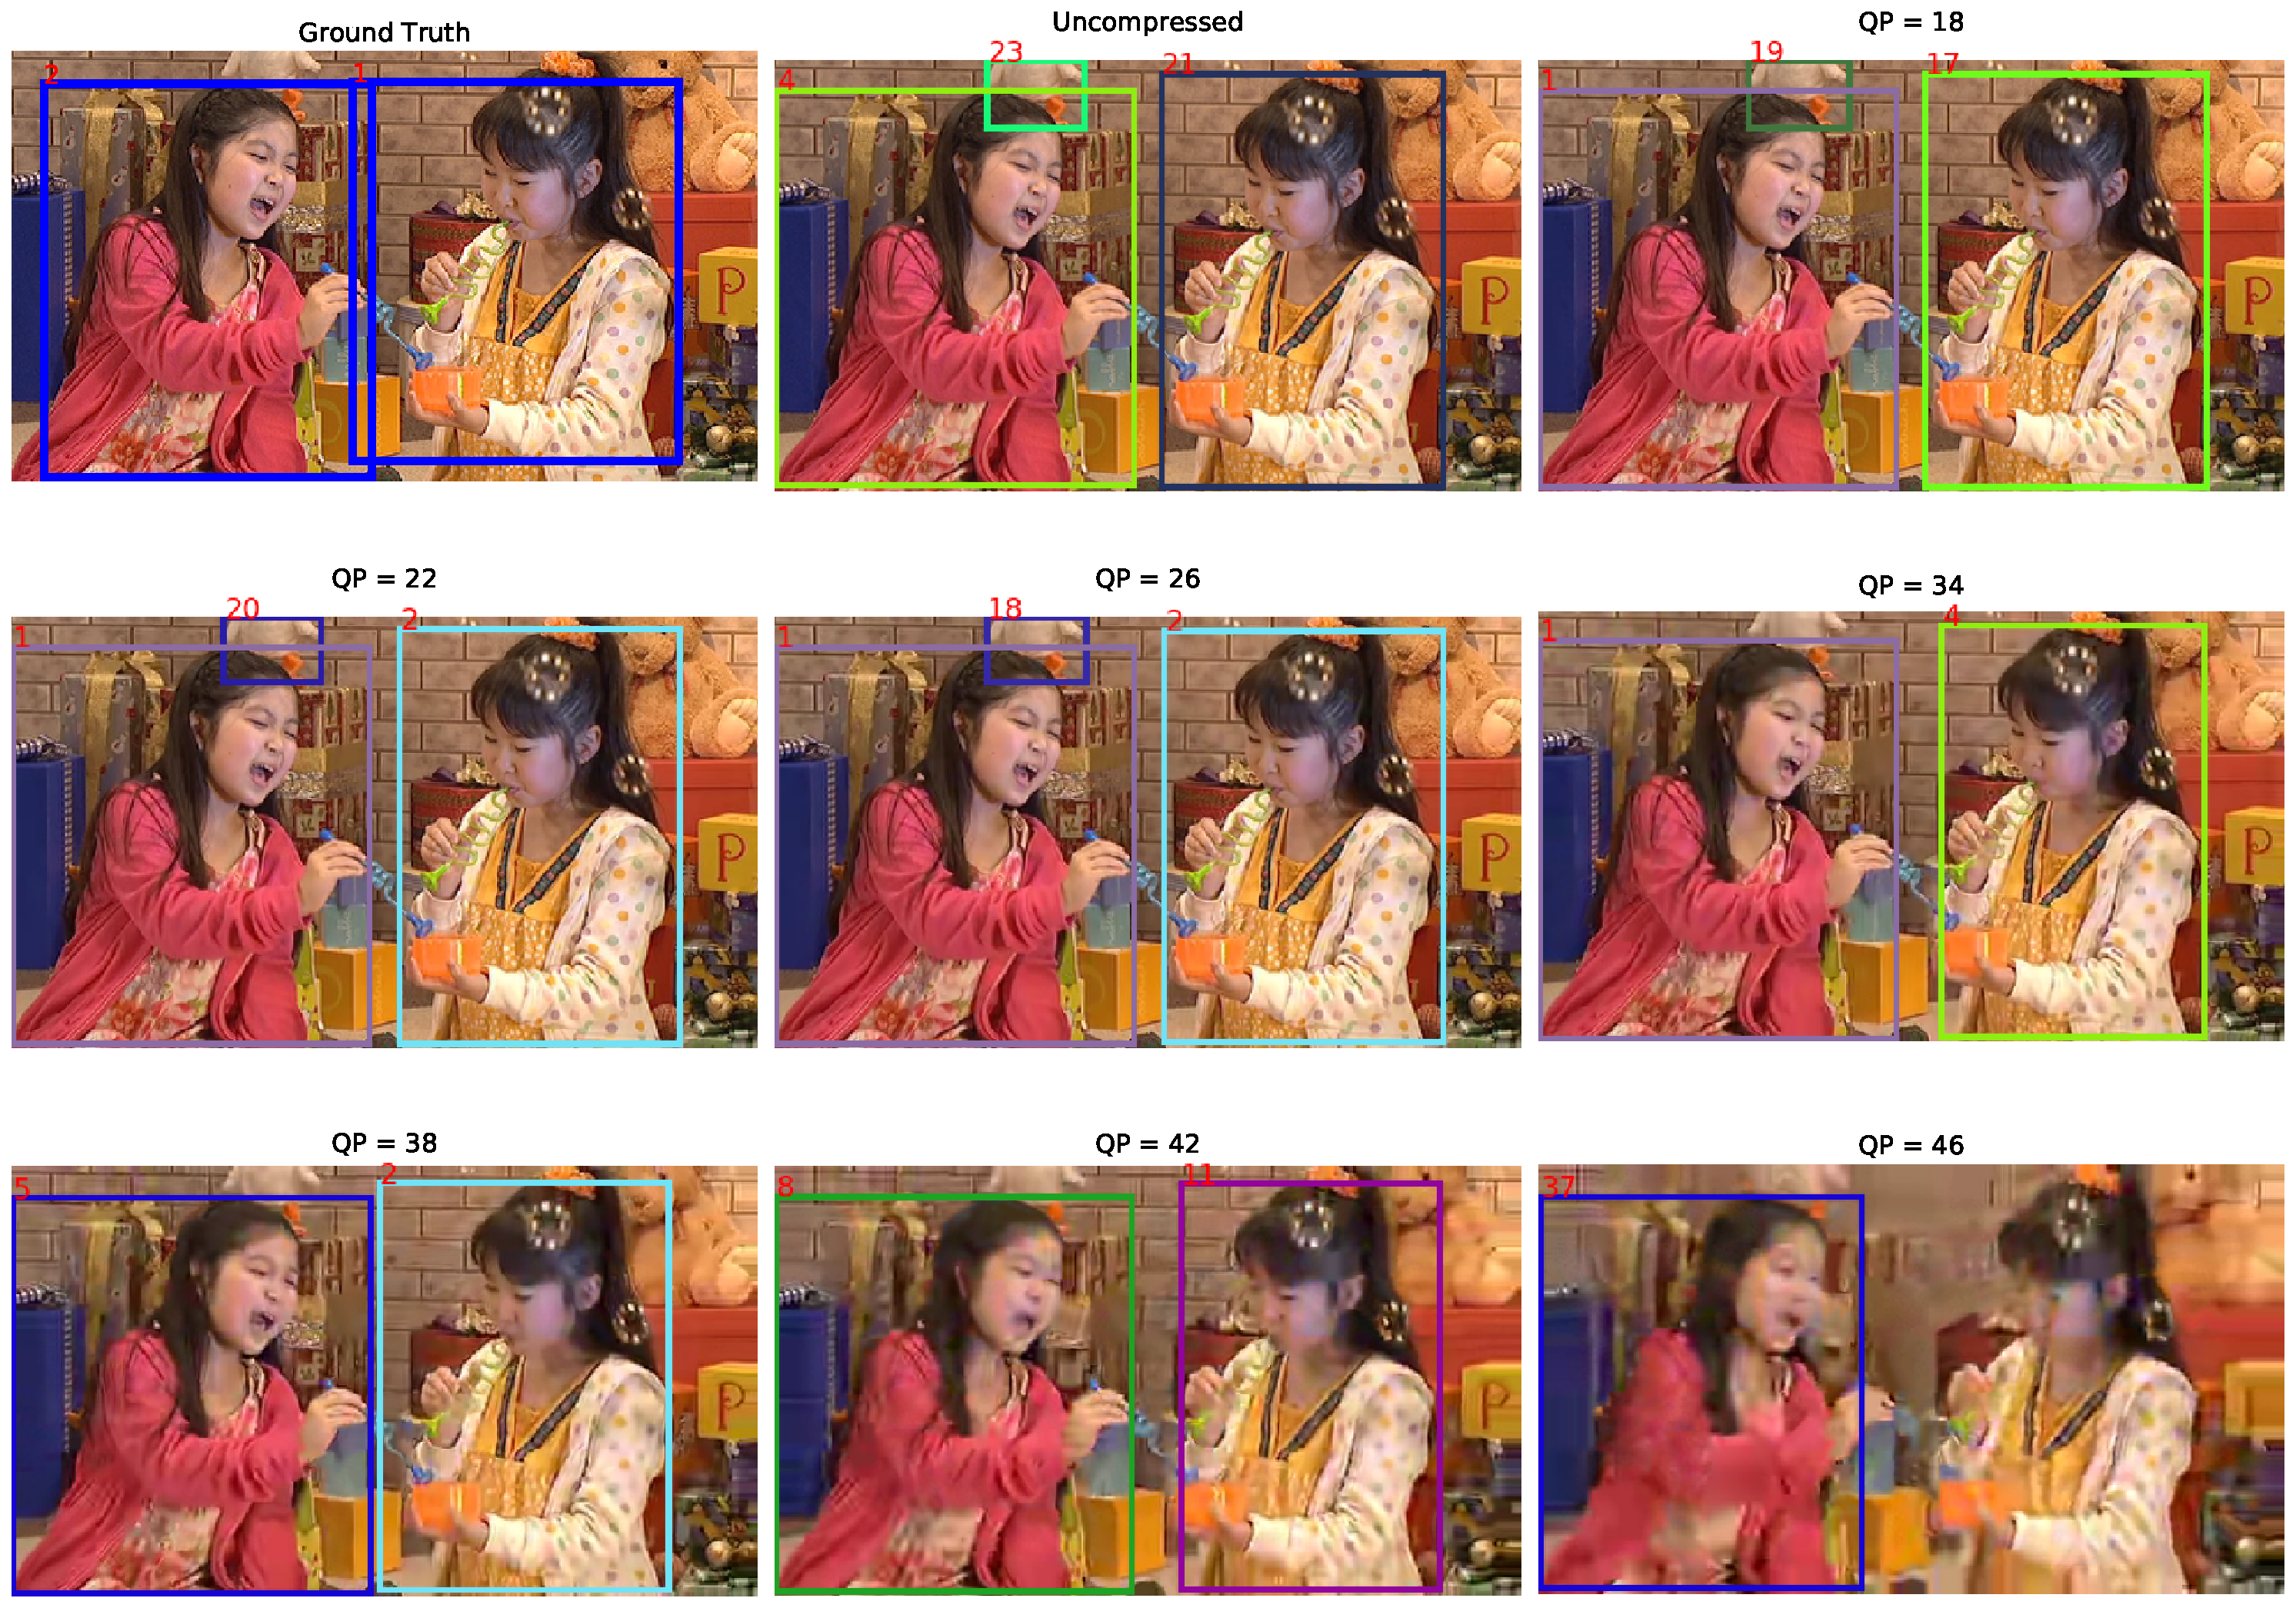
\includegraphics[width=1.0\linewidth]{img/BlowingBubbles_0_frame465.pdf}
  \caption[Comparison of Class D BlowingBubbles image frames at 465 at different QP]
  {
  Comparison of Class D BlowingBubbles image frames at 465 at different QP.
  }
  \label{fig:BlowingBubbles_0_frame465}
\end{figure}
This reveals that the detector incorrectly detects and recognizes this object as "person" at the lower QP, but as the image quality drops at the higher QP, the detector starts to not detect this particular object. Note that this toy object is not a part of the ground truth. This outcome was also observed in the other frames as well. This observation illustrates that as QP increases, FP may decrease, leading to increased MOTA. In this sequence. after QP = 38, the image quality further drops, and as shown in Figure \ref{fig:BlowingBubbles_0_frame465}, one "person" object is not detected at QP = 46, thereby FN increases. We observed that not only MOTA, the detection performance and ID measure also behave in the same way such that the performance scores increase up to the middle of the QP range and decrease thereafter. Though there is no occlusion in this sequence, we observed IDs increasing due to the drop of the image quality that causes "gap" in a trajectory similar to the outcome in Johnny.


\subsection{Cactus}
Here, we will present the analysis of tracking results in this sequence, where "potted plant" is the only object. Similar to BlowingBubbles, we observed an increase of MOTA and F1 in the middle of the QP range, as shown in Figure \ref{fig:Cactus_58_multiplots_qp}. Table \ref{tab:Cactus_58} shows the corresponding numerical results. To explain this result, we inspected the video sequence frame by frame and compared various QP cases at frame 32, as shown in Figure \ref{fig:Cactus_58_frame032}.
\begin{figure}[!htbp]
  \centering
  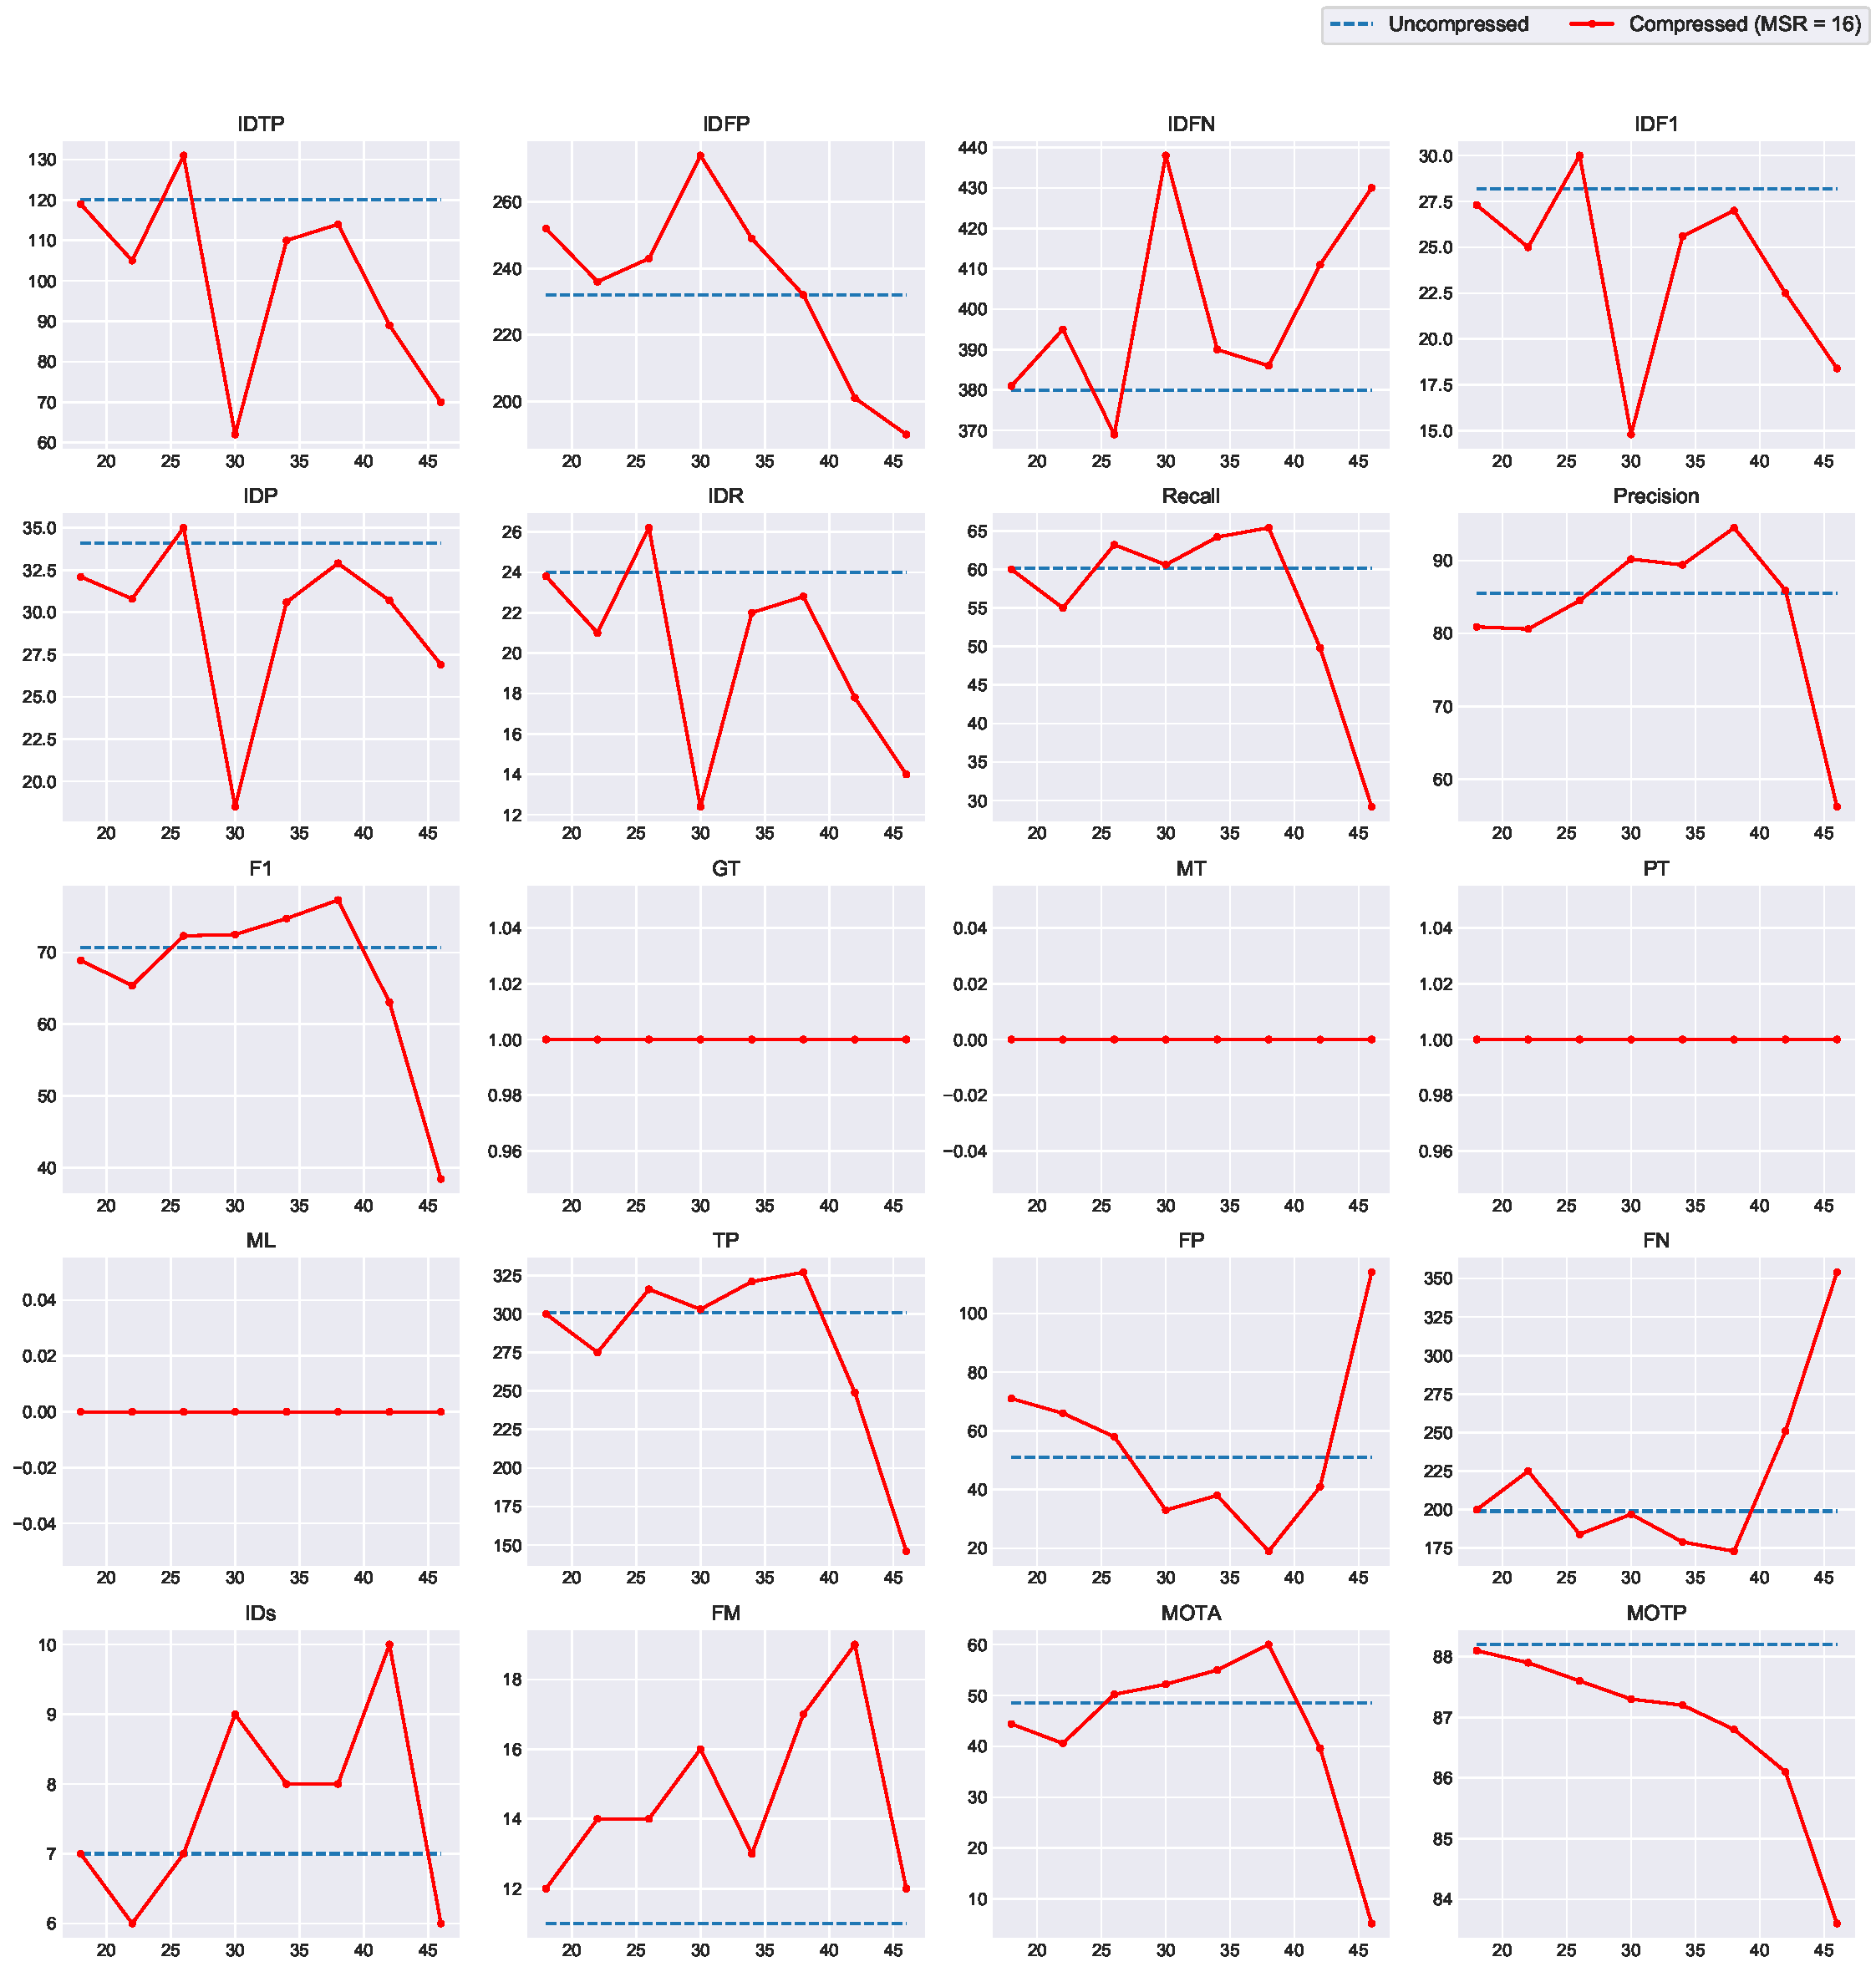
\includegraphics[width=1.0\linewidth]{img/Cactus_58_multiplots_qp.pdf}
  \caption[Visualization of the performance results in Class B Cactus at different QP]
  {
     Visualization of the performance results in Class B Cactus at different QP.
  }
  \label{fig:Cactus_58_multiplots_qp}
\end{figure}
\begin{table}[!tb]
    \centering
    \caption[Performance results on Cactus]
    {Performance results on Cactus.}
    \resizebox{1.0\linewidth}{!}{
\begin{tabular}{llrrrrrrrrrrrrrrrrrrrr}
\toprule
          QP &          MSR &   IDTP &   IDFP &   IDFN &  IDF1 &   IDP &   IDR &  Recall &  Precision &    F1 &  GT &  MT &  PT &  ML &  TP &  FP &  FN &  IDs &  FM &  MOTA &  MOTP \\
\midrule
Uncompressed & Uncompressed & 120.00 & 232.00 & 380.00 & 28.20 & 34.10 & 24.00 &   60.20 &      85.50 & 70.65 &   1 &   0 &   1 &   0 & 301 &  51 & 199 &    7 &  11 & 48.60 & 88.20 \\
          18 &           16 & 119.00 & 252.00 & 381.00 & 27.30 & 32.10 & 23.80 &   60.00 &      80.90 & 68.90 &   1 &   0 &   1 &   0 & 300 &  71 & 200 &    7 &  12 & 44.40 & 88.10 \\
          22 &           16 & 105.00 & 236.00 & 395.00 & 25.00 & 30.80 & 21.00 &   55.00 &      80.60 & 65.38 &   1 &   0 &   1 &   0 & 275 &  66 & 225 &    6 &  14 & 40.60 & 87.90 \\
          26 &           16 & 131.00 & 243.00 & 369.00 & 30.00 & 35.00 & 26.20 &   63.20 &      84.50 & 72.31 &   1 &   0 &   1 &   0 & 316 &  58 & 184 &    7 &  14 & 50.20 & 87.60 \\
          30 &           16 &  62.00 & 274.00 & 438.00 & 14.80 & 18.50 & 12.40 &   60.60 &      90.20 & 72.49 &   1 &   0 &   1 &   0 & 303 &  33 & 197 &    9 &  16 & 52.20 & 87.30 \\
          34 &           16 & 110.00 & 249.00 & 390.00 & 25.60 & 30.60 & 22.00 &   64.20 &      89.40 & 74.73 &   1 &   0 &   1 &   0 & 321 &  38 & 179 &    8 &  13 & 55.00 & 87.20 \\
          38 &           16 & 114.00 & 232.00 & 386.00 & 27.00 & 32.90 & 22.80 &   65.40 &      94.50 & 77.30 &   1 &   0 &   1 &   0 & 327 &  19 & 173 &    8 &  17 & 60.00 & 86.80 \\
          42 &           16 &  89.00 & 201.00 & 411.00 & 22.50 & 30.70 & 17.80 &   49.80 &      85.90 & 63.05 &   1 &   0 &   1 &   0 & 249 &  41 & 251 &   10 &  19 & 39.60 & 86.10 \\
          46 &           16 &  70.00 & 190.00 & 430.00 & 18.40 & 26.90 & 14.00 &   29.20 &      56.20 & 38.43 &   1 &   0 &   1 &   0 & 146 & 114 & 354 &    6 &  12 &  5.20 & 83.60 \\
\bottomrule
\end{tabular}
    }
    \label{tab:Cactus_58}
\end{table}
\begin{figure}[!htbp]
  \centering
  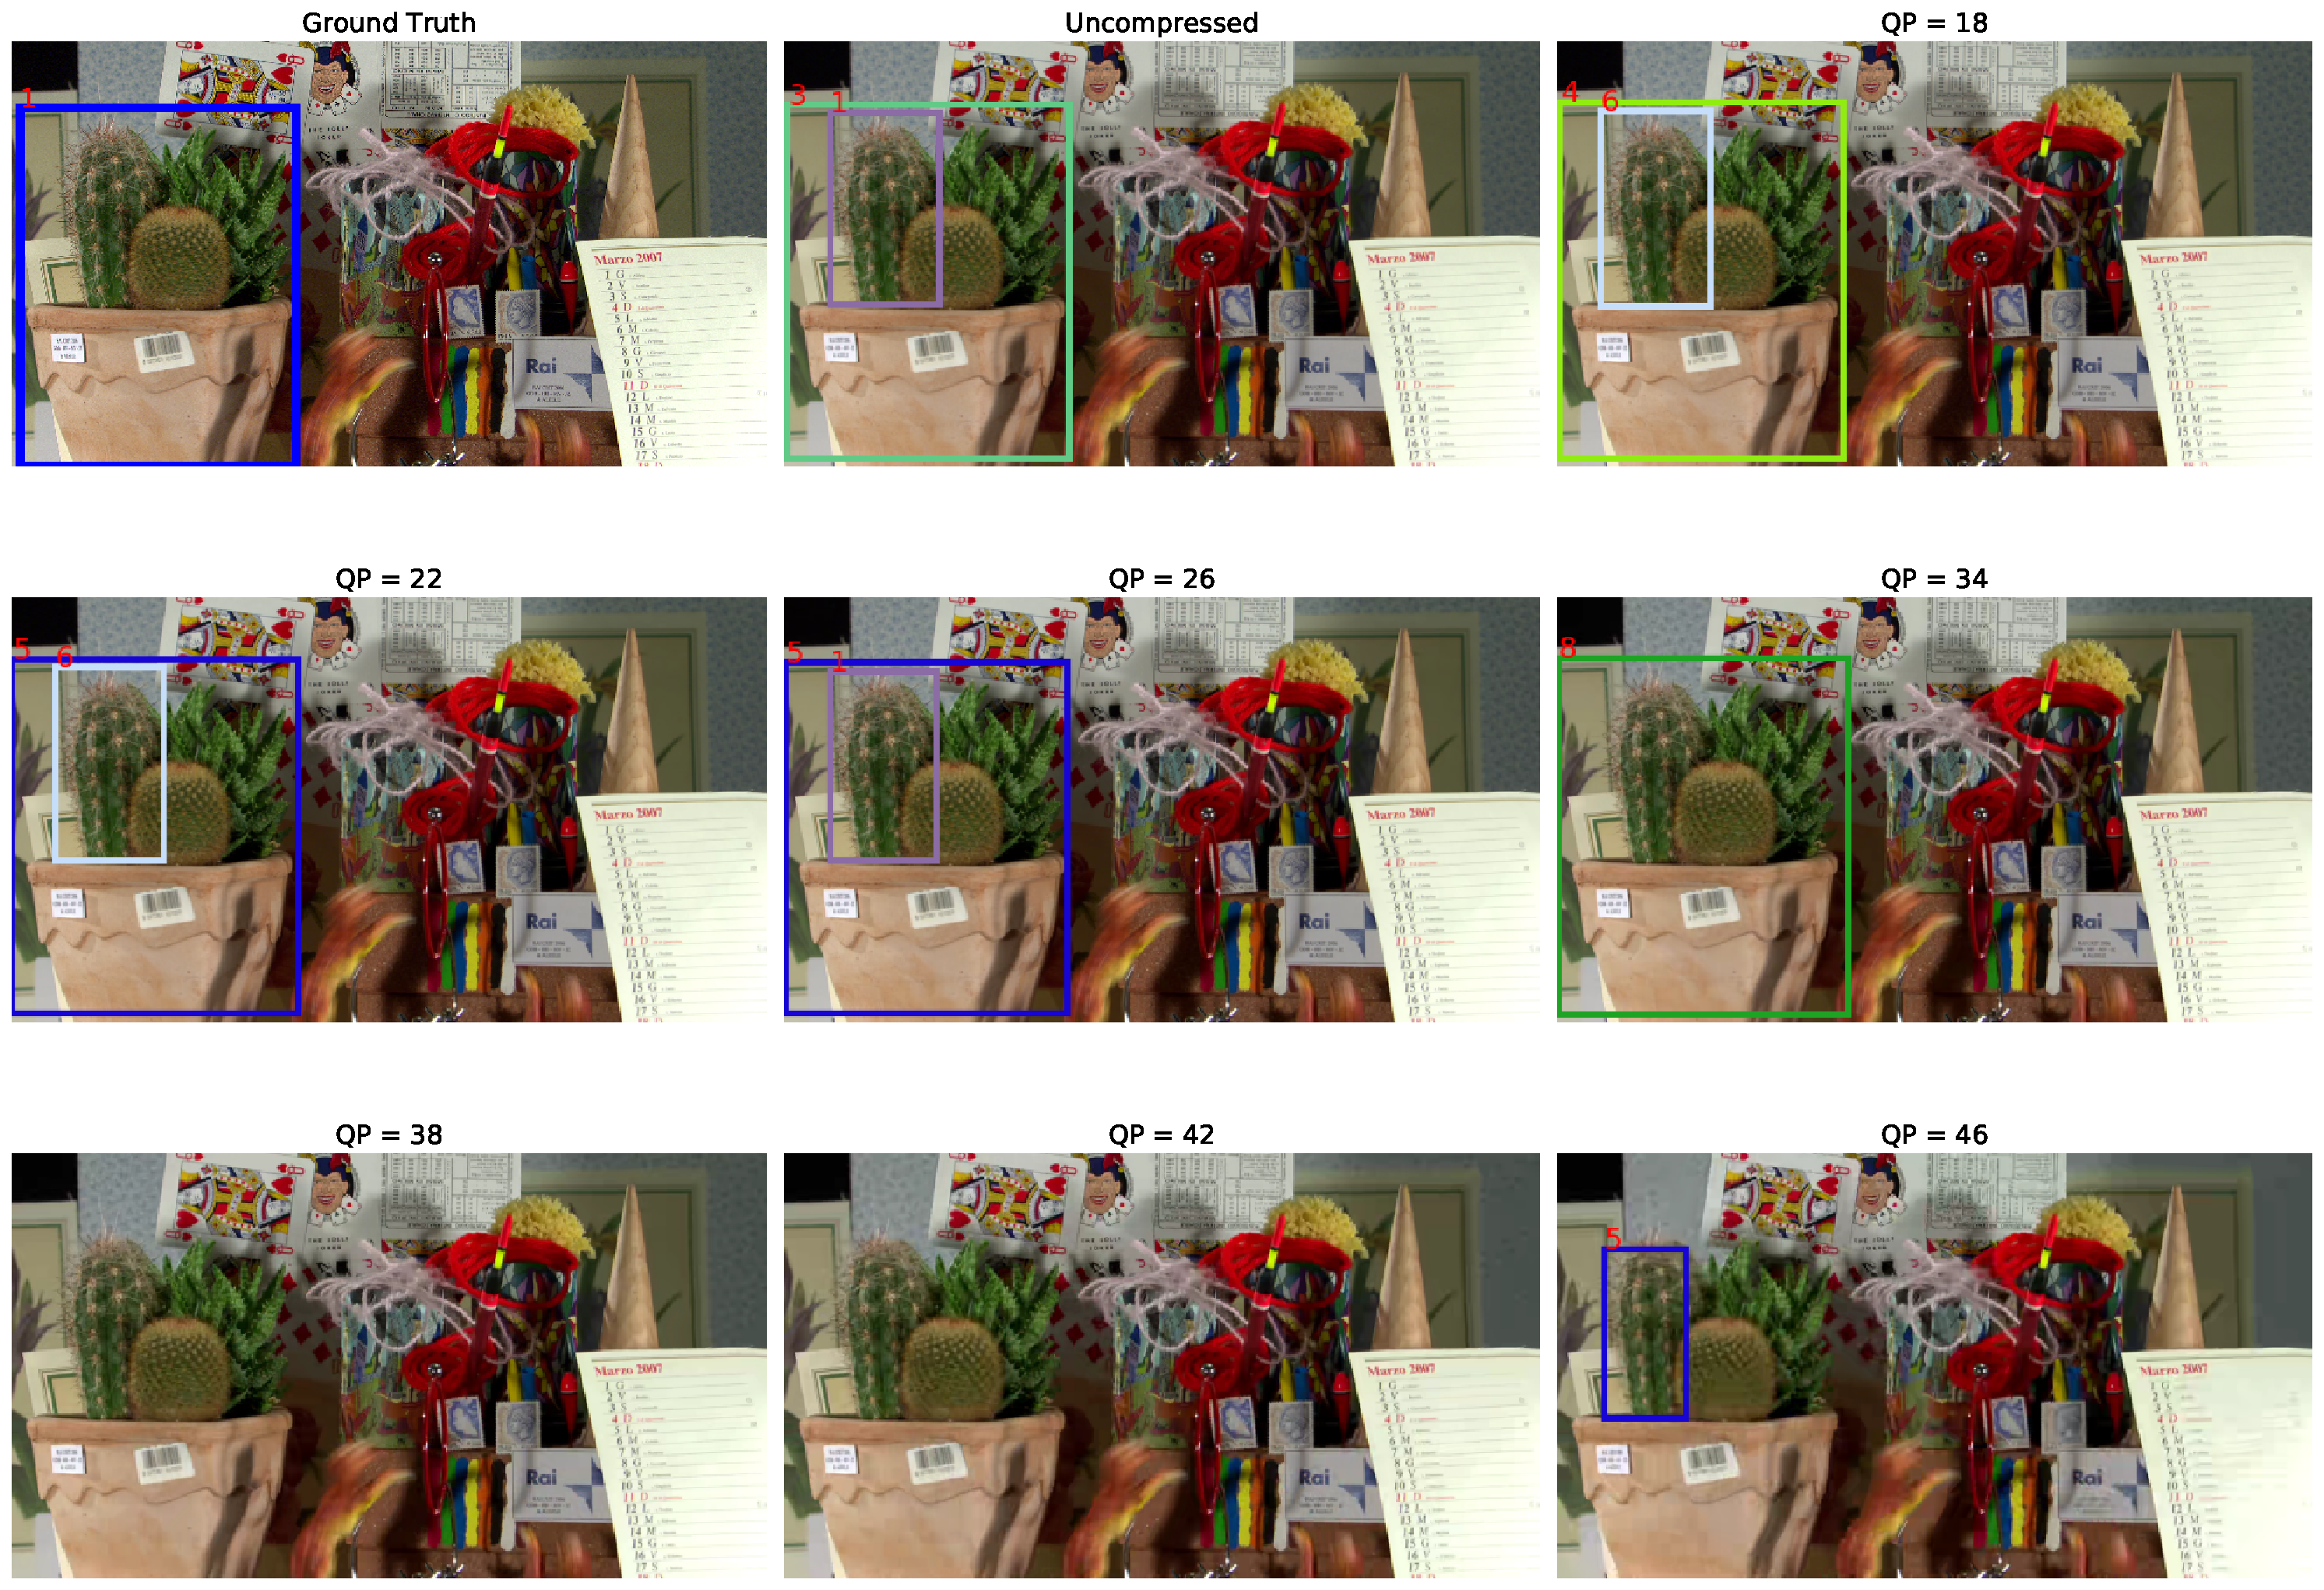
\includegraphics[width=1.0\linewidth]{img/Cactus_58_frame032.pdf}
  \caption[Comparison of Class B Cactus image frames at 32 among different QP]
  {
    Comparison of Class B Cactus image frames at 32 at different QP.
  }
  \label{fig:Cactus_58_frame032}
\end{figure}
From this comparison, we observed that YOLOv3 incorrectly detect two objects at a single target until QP = 26. Ground truth only contains one "potted plant" object. At QP = 34, we can see the correctly detected object, but as QP increases further, the object is no longer detected and at QP = 46, YOLOv3 detected a wrong target. This illustrates the decrease of FP midway through the QP range and its increase again at high QP. It is also observed that FN decreases slightly at the middle of the QP range but increases at high QP, since the correct target is no longer detected. In fact, not only at frame 32, but we also observed similar outcomes in other frames. This reveals that the cause of an increase of MOTA midway through the QP range is due to the decrease of FP and FN. One reason for the outcome we observed at frame 32 could be that the type of object is problematic because there are three cactuses in a vase, so YOLOv3 incorrectly detect one of the cactuses as a "potted plant" instead of detecting all three cactuses in a vase as a "potted plant".


\subsection{Discussion}
We inspected the four individual video sequences to gain the better insight into the general tracking performance measured by MOTA. From the inspected video samples, we found that MOTA scores in BasketballPass and Johnny are consistent with the expectation that tracking performance decreases as QP increases. However, the MOTA scores in BlowingBubbles and Cactus increase midway through the QP range and decrease thereafter. We found that these results are due to the type of object that makes the YOLOv3 detector incorrectly detect wrong targets, and FP was observed to be high even in the uncompressed video. Recall that we are using SORT based on YOLOv3, so the tracking performance is dependent on the detection performance. Note that since FP was high in the uncompressed sequence, as QP increases and the image quality drops, FP was observed to decrease. This insight also explains why we observed an increase in Precision in the average results. From Equation \eqref{eqn:Precision}, Precision depends on TP and FP, and since FP decreases in some video samples, Precision was observed to increase.

Not only does the tracking performance depend on the quality of the detector, but it also depends on the quality of the tracker. Re-ID for the long-term undetection and occlusion is not implemented in our tracker, SORT, so it affects the ID measure and IDs.

Finally, for the MOTP metric, we observed an increase of MOTP with increasing QP in some sequences: BasketballPass, Johnny, and BlowingBubbles. Since MOTP measures how well the objects are localized relative to the ground truth, the results from individual sequences tell us that object localization improves midway through the QP range, but decreases thereafter as the image quality further drops. Not all the video sequences behave in this way, but these outcomes contributed to the average results.